\documentclass{beamer}
\usepackage[utf8]{inputenc}
\usepackage[spanish]{babel}
\usepackage{graphicx}
\usepackage{tikz}
\usepackage{svg}

% Tema con navegación
\usetheme{Berlin}
\usecolortheme{default}
\useinnertheme{rounded}
\useoutertheme{smoothbars}
\usefonttheme{professionalfonts}
\usetikzlibrary{shapes.geometric}

% Color exacto del fondo
\definecolor{viuorangeexact}{HTML}{ED4800}
\definecolor{myorange}{HTML}{E64E0D}

\setbeamercolor{frametitle}{bg=myorange, fg=white}
\setbeamercolor{block title}{bg=myorange, fg=white}
\setbeamercolor{block body}{bg=white, fg=black}
\setbeamercolor{structure}{fg=viuorangeexact}
\setbeamercolor{title}{fg=white,bg=viuorangeexact}
\setbeamercolor{item}{fg=viuorangeexact}
\setbeamercolor{block title}{bg=myorange, fg=white}
\setbeamercolor{section in toc}{fg=viuorangeexact}
\setbeamercolor{palette primary}{bg=myorange, fg=white}
\setbeamercolor{palette secondary}{bg=myorange, fg=white}
\setbeamercolor{palette tertiary}{bg=myorange, fg=white}

% Fondo personalizado
\setbeamertemplate{background}{%
  \begin{tikzpicture}
    \useasboundingbox (0,0) rectangle (\paperwidth,\paperheight);
    \node[anchor=south west, inner sep=0pt] at (-3.0cm,0cm)
      {
\includegraphics[width=\paperwidth,height=\paperheight]{images/base.png}};
  \end{tikzpicture}%
}

\setbeamertemplate{itemize item}{%
  \tikz[baseline=-0.6ex]{\fill[black] (0,0) -- ++(0.2em,0.2em) -- ++(-0.2em,0.2em) -- ++(-0.2em,-0.2em) -- cycle;}%
}

\setbeamertemplate{itemize subitem}{%
  \tikz[baseline=-0.6ex]{\fill[black] (0,0) -- ++(0.2em,0.2em) -- ++(-0.2em,0.2em) -- ++(-0.2em,-0.2em) -- cycle;}%
}

\setbeamertemplate{itemize subsubitem}{%
  \tikz[baseline=-0.6ex]{\fill[black] (0,0) -- ++(0.2em,0.2em) -- ++(-0.2em,0.2em) -- ++(-0.2em,-0.2em) -- cycle;}%
}

\setbeamertemplate{enumerate item}{%
  \tikz[baseline=(char.base)]{
    \node[shape=diamond, fill=black, text=white, inner sep=1pt, minimum size=1.4em] (char) {\normalsize\insertenumlabel};
  }%
}

\makeatletter
\newcommand{\currentsectionindex}{0}
\newcommand{\sectionagenda}[2]{%
  \ifnum#1=\currentsectionindex\relax
    \item[{\tikz[baseline=(char.base)]{\node[shape=diamond, fill=black, text=white, inner sep=1pt, minimum size=1.4em] (char) {\normalsize #1};}}] {\color{structure}\textbf{#2}}%
  \else
    \item[{\tikz[baseline=(char.base)]{\node[shape=diamond, fill=black, text=white, inner sep=1pt, minimum size=1.4em] (char) {\normalsize #1};}}] {\color{gray}#2}%
  \fi
}

\setbeamertemplate{section in toc}{%
  \leavevmode%
  \hbox{% 
    \begin{tikzpicture}[baseline=(textnode.base)]
      \node[draw=none, fill=black, minimum size=1.4em, inner sep=0pt, shape=rectangle, rotate=45] (diamond) {};
      \node[inner sep=0pt, text=white] (textnode) at (diamond.center) {\strut\inserttocsectionnumber};
    \end{tikzpicture}%
  }~\inserttocsection\par%
}
\setbeamertemplate{section number projected}{} 
\makeatother

% Agenda dinámica por sección
\AtBeginSection[]{%
  \begin{frame}
    \frametitle{Agenda}
    \begin{columns}
      \column{2cm}
      \column{10cm}
      \begin{itemize}
        \setlength{\itemsep}{0.4em}
        \sectionagenda{1}{Introducción}
        \sectionagenda{2}{Estado del Arte}
        \sectionagenda{3}{Materiales}
        \sectionagenda{4}{Métodos}
        \sectionagenda{5}{Resultados}
        \sectionagenda{6}{Conclusiones}
        \sectionagenda{7}{Limitaciones}
        \sectionagenda{8}{Trabajos futuros}
      \end{itemize}
    \end{columns}
  \end{frame}%
}

\AtBeginSubsection[] {
  \begin{frame}[t]
    \frametitle{Contenido de la sección}
    \tableofcontents[sectionstyle=show/hide,subsectionstyle=show/shaded/hide]
  \end{frame}
}


% Datos del proyecto
\title{Generación de Música Personalizada\\ a través de Modelos Generativos Adversariales}
\author[Rafael Luque Tejada]{Autor: Rafael Luque Tejada\\Tutora: Dra. Yaneth Coromoto Romero Caldera}
\institute{%
Universidad Internacional de Valencia (VIU)\\Máster Universitario en Inteligencia Artificial}
\date{Curso 2024--2025}
\titlegraphic{
\includegraphics[width=3cm]{images/viu_logo.png}}

\begin{document}

\frame{\titlepage}

% Agenda
\section*{Agenda}
\begin{frame}
  \frametitle{Agenda}
  \begin{columns}
    \column{2cm}
    \column{10cm}
    \begin{itemize}
      \setlength{\itemsep}{0.4em}
      \sectionagenda{1}{Introducción}
      \sectionagenda{2}{Estado del Arte}
      \sectionagenda{3}{Materiales}
      \sectionagenda{4}{Métodos}
      \sectionagenda{5}{Resultados}
      \sectionagenda{6}{Conclusiones}
      \sectionagenda{7}{Limitaciones}
      \sectionagenda{8}{Trabajos futuros}
    \end{itemize}
  \end{columns}
\end{frame}%


\renewcommand{\currentsectionindex}{1}
\section{Introducción}
\begin{frame}{Introducción}
\begin{columns}
\column{5.5cm}
\begin{itemize}
  \item Planteamiento del problema
  \item Objetivos
  \item Justificación
  \item Alcance
\end{itemize}
\column{6cm}
\begin{figure}[H]
  \centering
  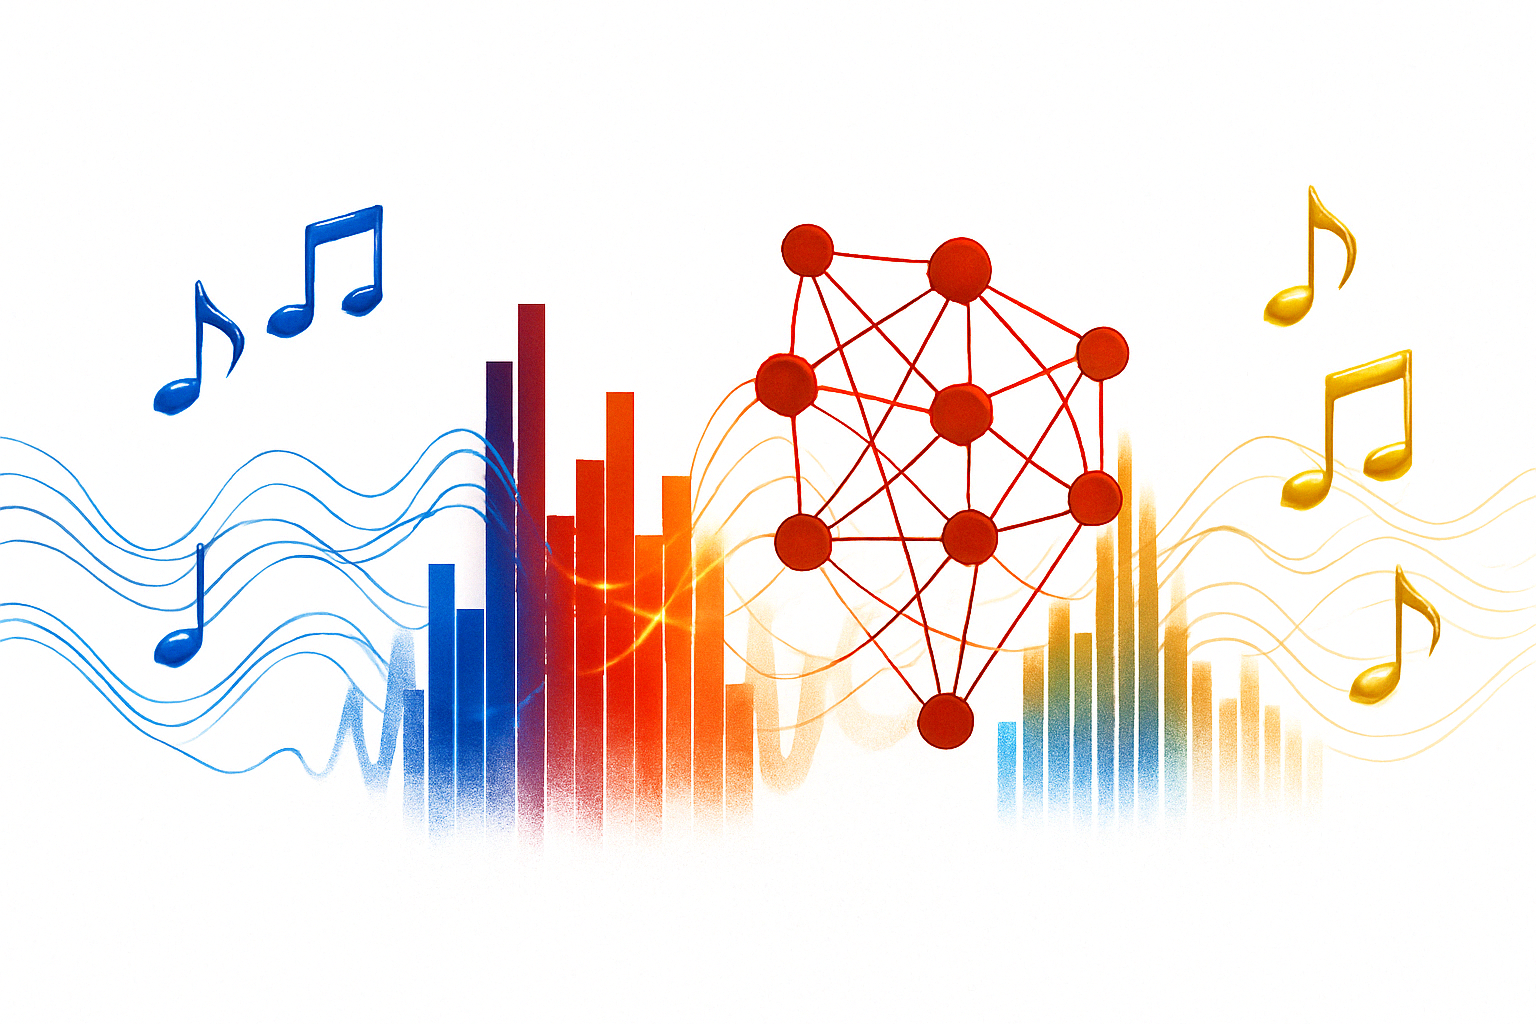
\includegraphics[width=0.85\textwidth]{images/data_introduction.png}
\end{figure}
\end{columns}
\end{frame}

\begin{frame}{Introducción}
  \begin{columns}
  \column{5.7cm}
  \begin{itemize}
    \item \textbf{Planteamiento del problema}
    \item Objetivos
    \item Justificación
    \item Alcance
  \end{itemize}
  \column{6cm}
  \end{columns}
  \end{frame}

  
\begin{frame}{Introducción}
\begin{columns}
\column{5.7cm}
\begin{itemize}
  \item \textbf{Planteamiento del problema}
  \item Objetivos
  \item Justificación
  \item Alcance
\end{itemize}
\column{6cm}
Podría una máquina:
\begin{itemize}
  \item ¿extraer patrones referenciales?
  \item ¿distinguir géneros musicales?
  \item ¿generar nuevas piezas musicales?
\end{itemize}
\end{columns}
\end{frame}

\begin{frame}{Introducción}
\begin{columns}
\column{5.5cm}
\begin{itemize}
  \item Planteamiento del problema
  \item \textbf{Objetivos}
  \item Justificación
  \item Alcance
\end{itemize}
\column{6cm}
\end{columns}
\end{frame}

\begin{frame}{Introducción}
  \begin{columns}
  \column{5.5cm}
  \begin{itemize}
    \item Planteamiento del problema
    \item \textbf{Objetivos}
    \item Justificación
    \item Alcance
  \end{itemize}
  \column{6cm}
  1º Recopilar ejemplos de \textbf{datos} correspondientes con piezas musicales representativas de un género musical y que estén \textbf{bien etiquetadas}.
  \end{columns}
\end{frame}


\begin{frame}{Introducción}
  \begin{columns}
  \column{5.5cm}
  \begin{itemize}
    \item Planteamiento del problema
    \item \textbf{Objetivos}
    \item Justificación
    \item Alcance
  \end{itemize}
  \column{6cm}
  2º Transformar esas piezas musicales en \textbf{estructuras de datos} analizables y computables.
  \end{columns}
\end{frame}

\begin{frame}{Introducción}
  \begin{columns}
  \column{5.5cm}
  \begin{itemize}
    \item Planteamiento del problema
    \item \textbf{Objetivos}
    \item Justificación
    \item Alcance
  \end{itemize}
  \column{6cm}
  3º Diseñar un modelo basado en Inteligencia Artificial que sea capaz de \textbf{extraer información} crítica para \textbf{distinguir} cuáles son los \textbf{patrones} que asignan una pieza musical a un \textbf{género} concreto.
  \end{columns}
\end{frame}

\begin{frame}{Introducción}
  \begin{columns}
  \column{5.5cm}
  \begin{itemize}
    \item Planteamiento del problema
    \item \textbf{Objetivos}
    \item Justificación
    \item Alcance
  \end{itemize}
  \column{6cm}
  4º \textbf{Evaluar} el modelo generador mediante métricas que se apliquen a los \textbf{datos de salida} generados.
  \end{columns}
\end{frame}
\begin{frame}{Introducción}
\begin{columns}
\column{5.5cm}
\begin{itemize}
  \item Planteamiento del problema
  \item Objetivos
  \item \textbf{Justificación}
  \item Alcance
\end{itemize}
\column{6cm}
\end{columns}
\end{frame}

\begin{frame}{Introducción}
  \begin{columns}
  \column{5.5cm}
  \begin{itemize}
    \item Planteamiento del problema
    \item Objetivos
    \item \textbf{Justificación}
    \item Alcance
  \end{itemize}
  \column{6cm}
  \begin{itemize}
    \item Reconocimiento
    \item Bibliotecas
    \item Análisis
    \item Educación (y ocio)
  \end{itemize}
  \end{columns}
\end{frame}

\begin{frame}{Introducción}
\begin{columns}
\column{5.5cm}
\begin{itemize}
  \item Planteamiento del problema
  \item Objetivos
  \item Justificación
  \item \textbf{Alcance}
\end{itemize}
\column{6cm}
\begin{itemize}
  \item hip hop
  \item jazz
  \item pop
  \item rock
  \item blues
\end{itemize}
\end{columns}
\end{frame}

\renewcommand{\currentsectionindex}{2}
\section{Estado del Arte}
\begin{frame}{Estado del Arte}
  \vspace{0.5cm} % desplaza hacia abajo
  \hspace{2cm}
  {\fontsize{10pt}{12pt}\selectfont

  \begin{tabular}{|p{4cm}|p{6cm}|}
  \hline
  \textbf{Autor y año} & \textbf{Título del trabajo} \\
  \hline
  Santiago, F. and García Fronti, J. & Estado del Arte - M72.1.09 Gestión y análisis de datos no estructurados \\
  \hline
  Telefónica Tech. & AI of Things (VI) - Inteligencia Artificial Generativa, creando música a ritmo de perceptrón \\
  \hline
  Blanco Bejarano, J.J. & IA en la creatividad: Explorando la generación de arte y música \\
  \hline
  Jin, C. et al. & A Transformer Generative Adversarial Network for MultiTrack Music Generation \\
  \hline
  \end{tabular}

  } % cierre del tamaño
\end{frame}

\renewcommand{\currentsectionindex}{3}
\section{Materiales}
\begin{frame}{Hardware}
    \begin{figure}[H]
      \centering
      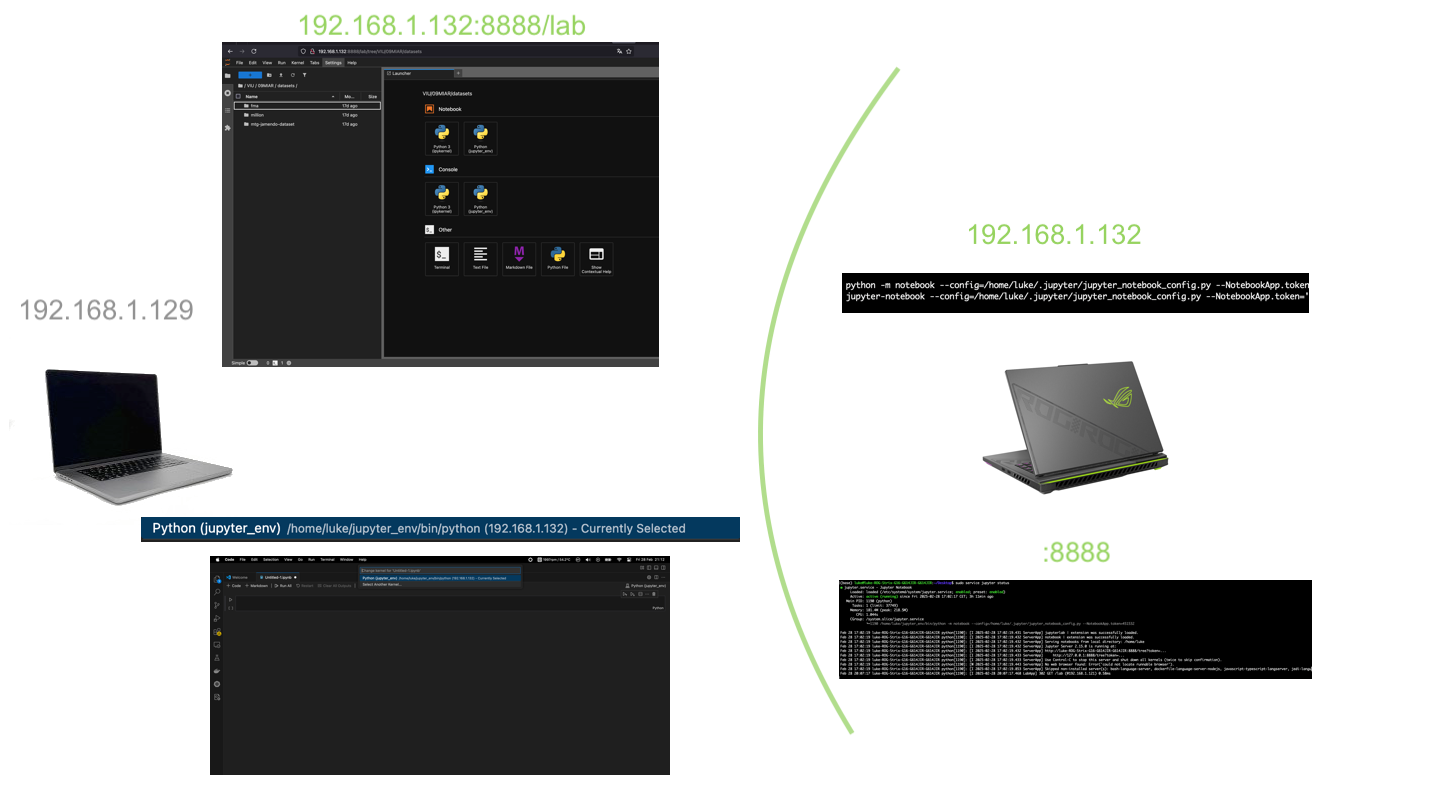
\includegraphics[width=0.85\textwidth]{images/jupyter-diagram.png}
    \end{figure}
    \begin{itemize}
      \item Ordenador \textbf{MacBook Pro 15 pulgadas, 2017.}
      \item Ordenador \textbf{Asus ROG Strix G16 G614JIR-N4004 - Gaming 16 pulgadas, 2024.}
      % \item Paper tablet \textbf{reMarkable 2.}
      % \item Calculadora \textbf{Texas Instruments TI-92 Plus.}
    \end{itemize}

\end{frame}

\begin{frame}{Software}
  \begin{itemize}
    \item VisualStudio Code. Versión 1.97.2.
    \item TextShop. Version 5.49 (5.49).
    \item Git. Versión 2.39.3 (Apple Git-145).
    \item Python Version: 3.12.7
    \item Librería de Ptyhon \emph{Torch}. Version: 2.6.0+cu124.
    \item CUDA Version: 12.4
  \end{itemize}
\end{frame}

\begin{frame}{Datasets}
\begin{itemize}
  \item FMA: Free Music Archive.
  \begin{itemize}
    \item \textbf{FMA Large:} 106,000 pistas, aproximadamente 100GB.
    \item 160 géneros
  \end{itemize}
  \item JAMENDO, Million Song Dataset
  \begin{itemize}
    \item 190 categorías de género
    \item más de 50,000 pistas
  \end{itemize}
  \item Million Song Dataset
  \begin{itemize}
    \item 15 categorías de género
    \item 1500 ficheros
  \end{itemize}
\end{itemize}
\end{frame}

\renewcommand{\currentsectionindex}{4}
\section{Métodos}
\begin{frame}{Metodología}
\begin{center}
  CRISP-ML(Q) + Scrum (integración ágil)
\end{center}
\begin{center}
  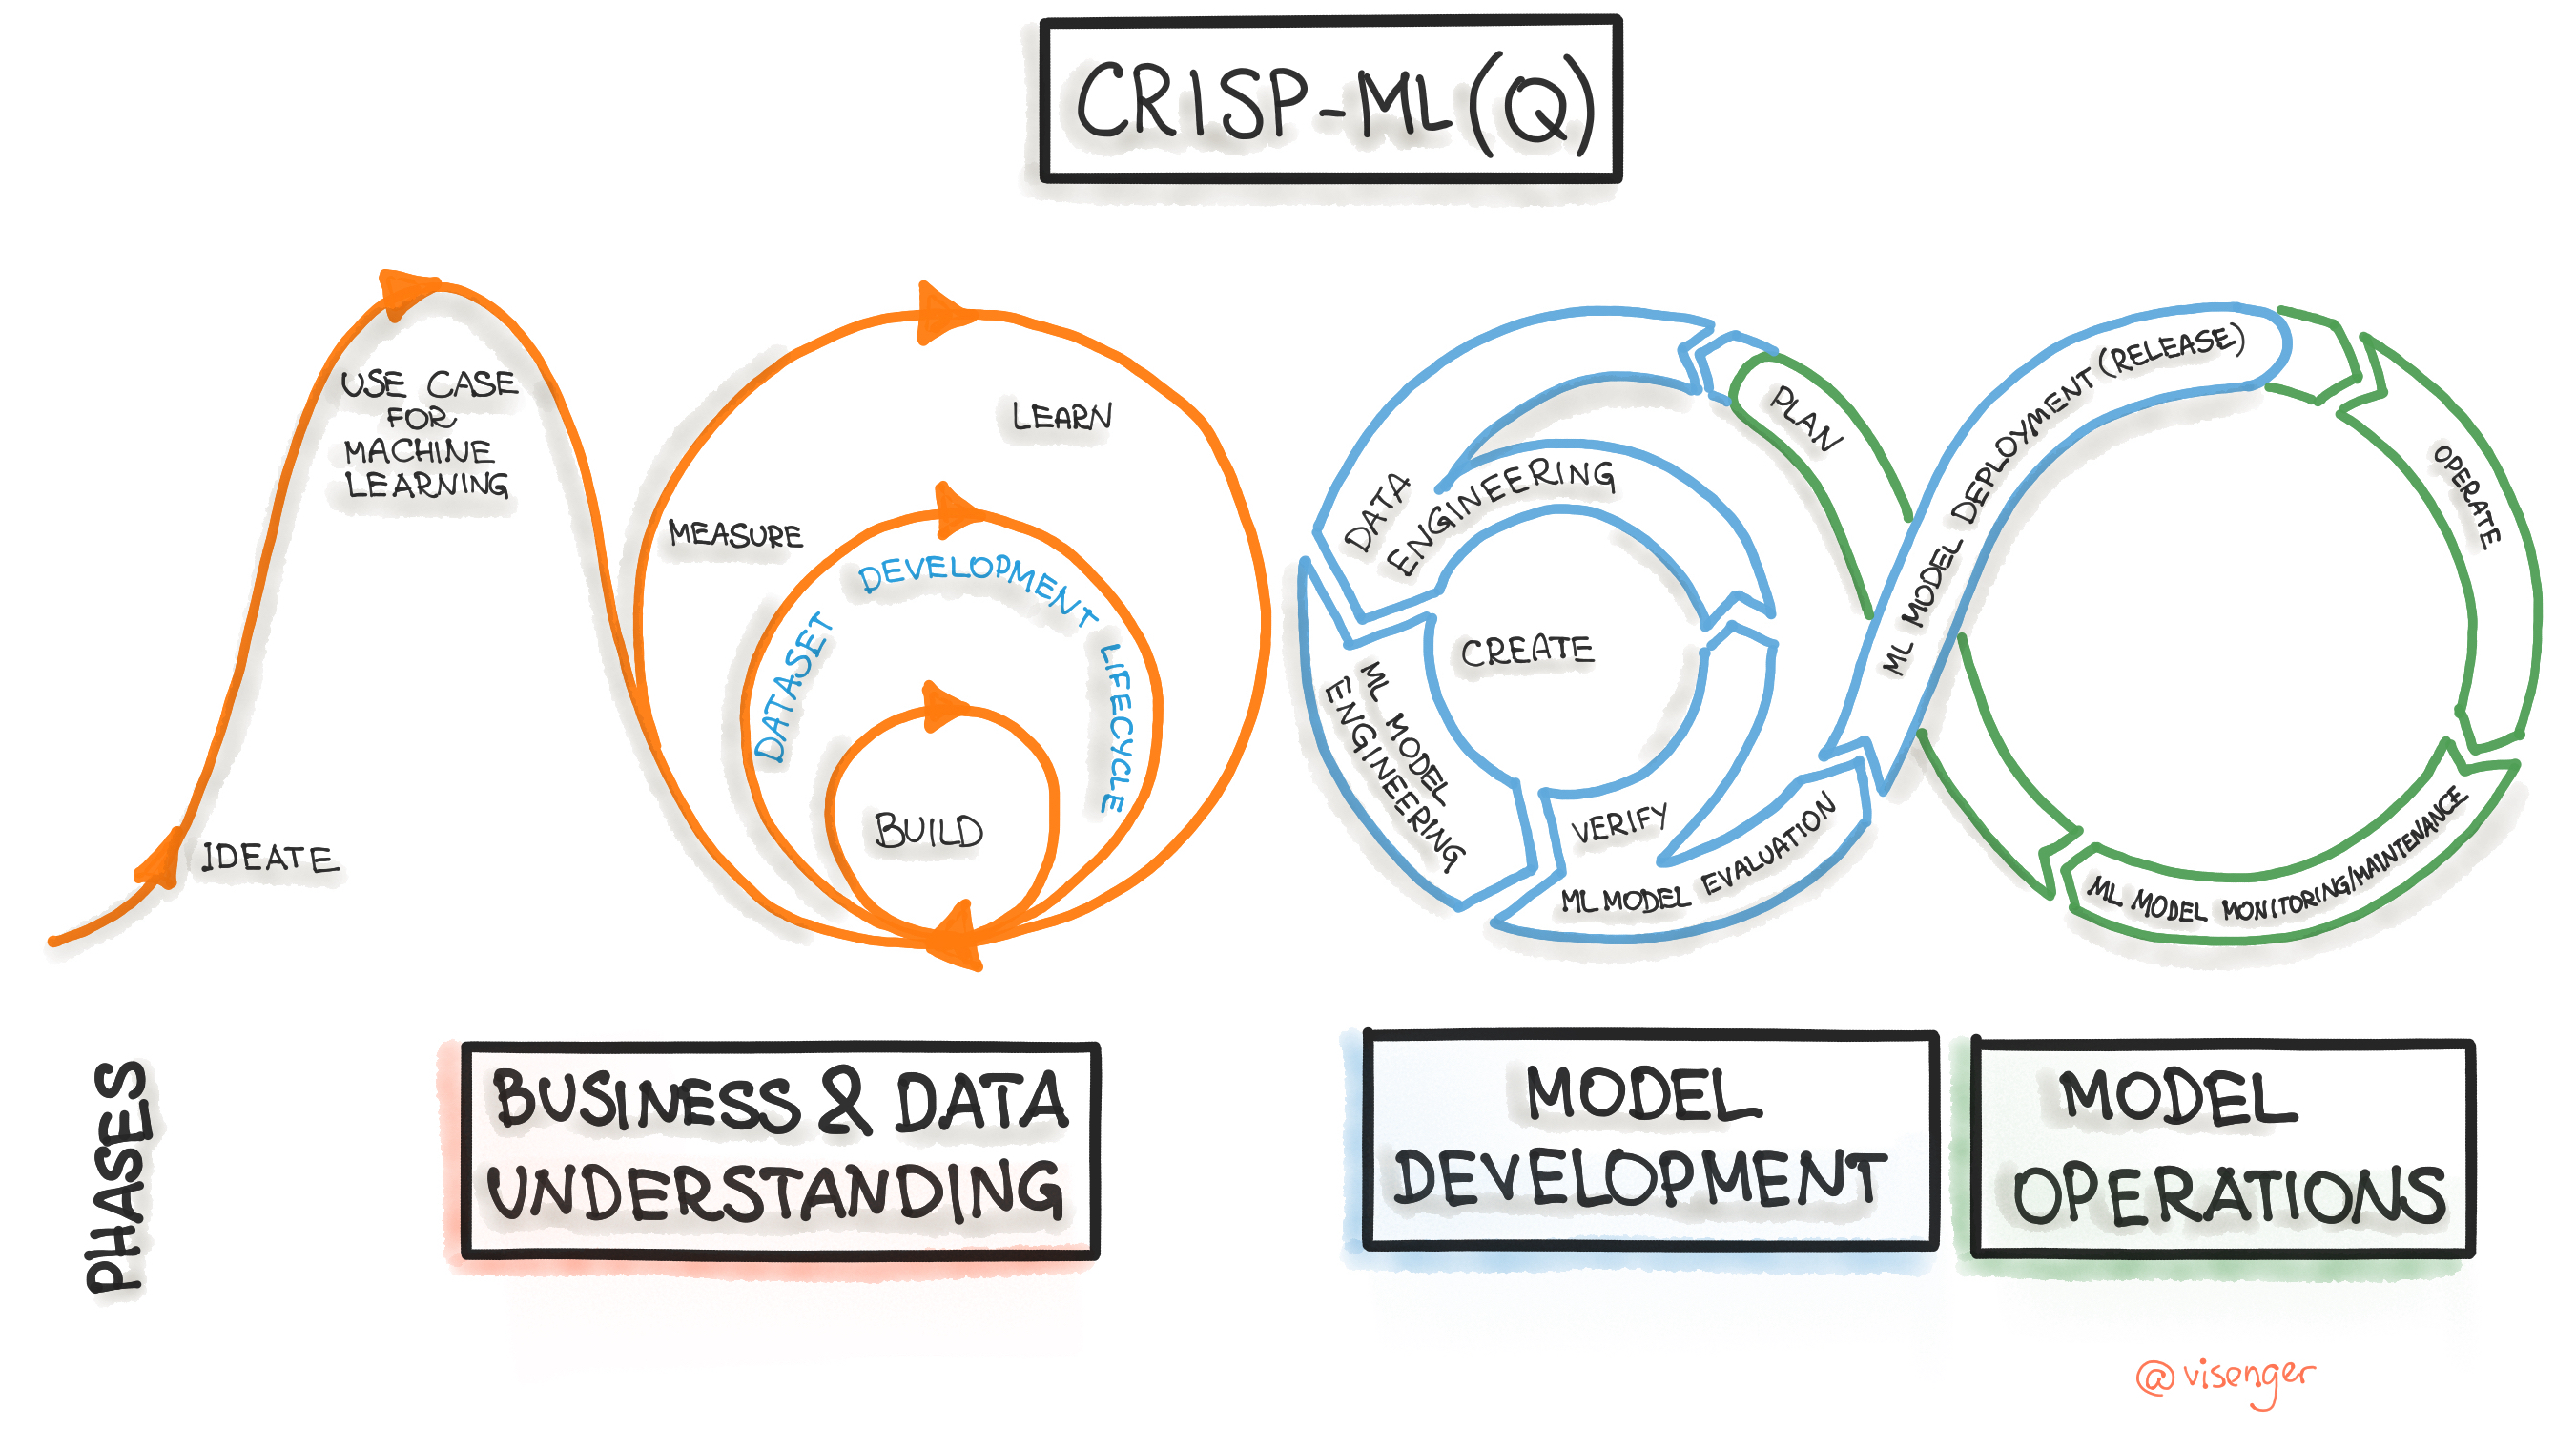
\includegraphics[width=0.85\textwidth]{images/crisp-ml-process.jpg}
\end{center}
\end{frame}

\begin{frame}{Metodología}
  \begin{enumerate}
    \item \textbf{Comprensión del negocio}.
    \item \textbf{Comprensión de los datos}.
    \item \textbf{Preparación de los datos}.
    \item \textbf{Modelado}.
    \item \textbf{Evaluación}.
    \item \textbf{Implementación y monitoreo}.
  \end{enumerate}
\end{frame}


\begin{frame}{Metodología}
  \begin{enumerate}
    \item \textbf{Comprensión del negocio}: Definir  problema y objetivos.
    \item \textbf{Comprensión de los datos}: Recopilación y exploración de datos.
    \item \textbf{Preparación de los datos}.
  \end{enumerate}
\end{frame}


\begin{frame}{Metodología}
  \begin{enumerate}
    \setcounter{enumi}{3}
    \item \textbf{Modelado}: UML. Desarrollo.
    \item \textbf{Evaluación}: Validación de métricas y análisis del rendimiento.
    \item \textbf{Implementación y monitoreo}: Despliegue y seguimiento en producción.
  \end{enumerate}
\end{frame}

\begin{frame}{Metodología}
  \begin{center}
    \textbf{Modelado}: UML. Desarrollo.
    \begin{itemize}
      \item Análisis del sistema: formalización y especificación de requisitos. Diagramas de caso de uso.
      \item Especificación del modelo de clases
      \item Diagramas de Secuencia
      \item Especificación de Requisitos de la Interfaz
      \item Diseño de clases
      \item Diagrama de Paquetes
      \item Diseño de la interfaz
    \end{itemize}
  \end{center}
\end{frame}

\begin{frame}{Metodología}
  \begin{center}
    \textbf{Modelado}: UML. Desarrollo.
  \end{center}
  \begin{center}
    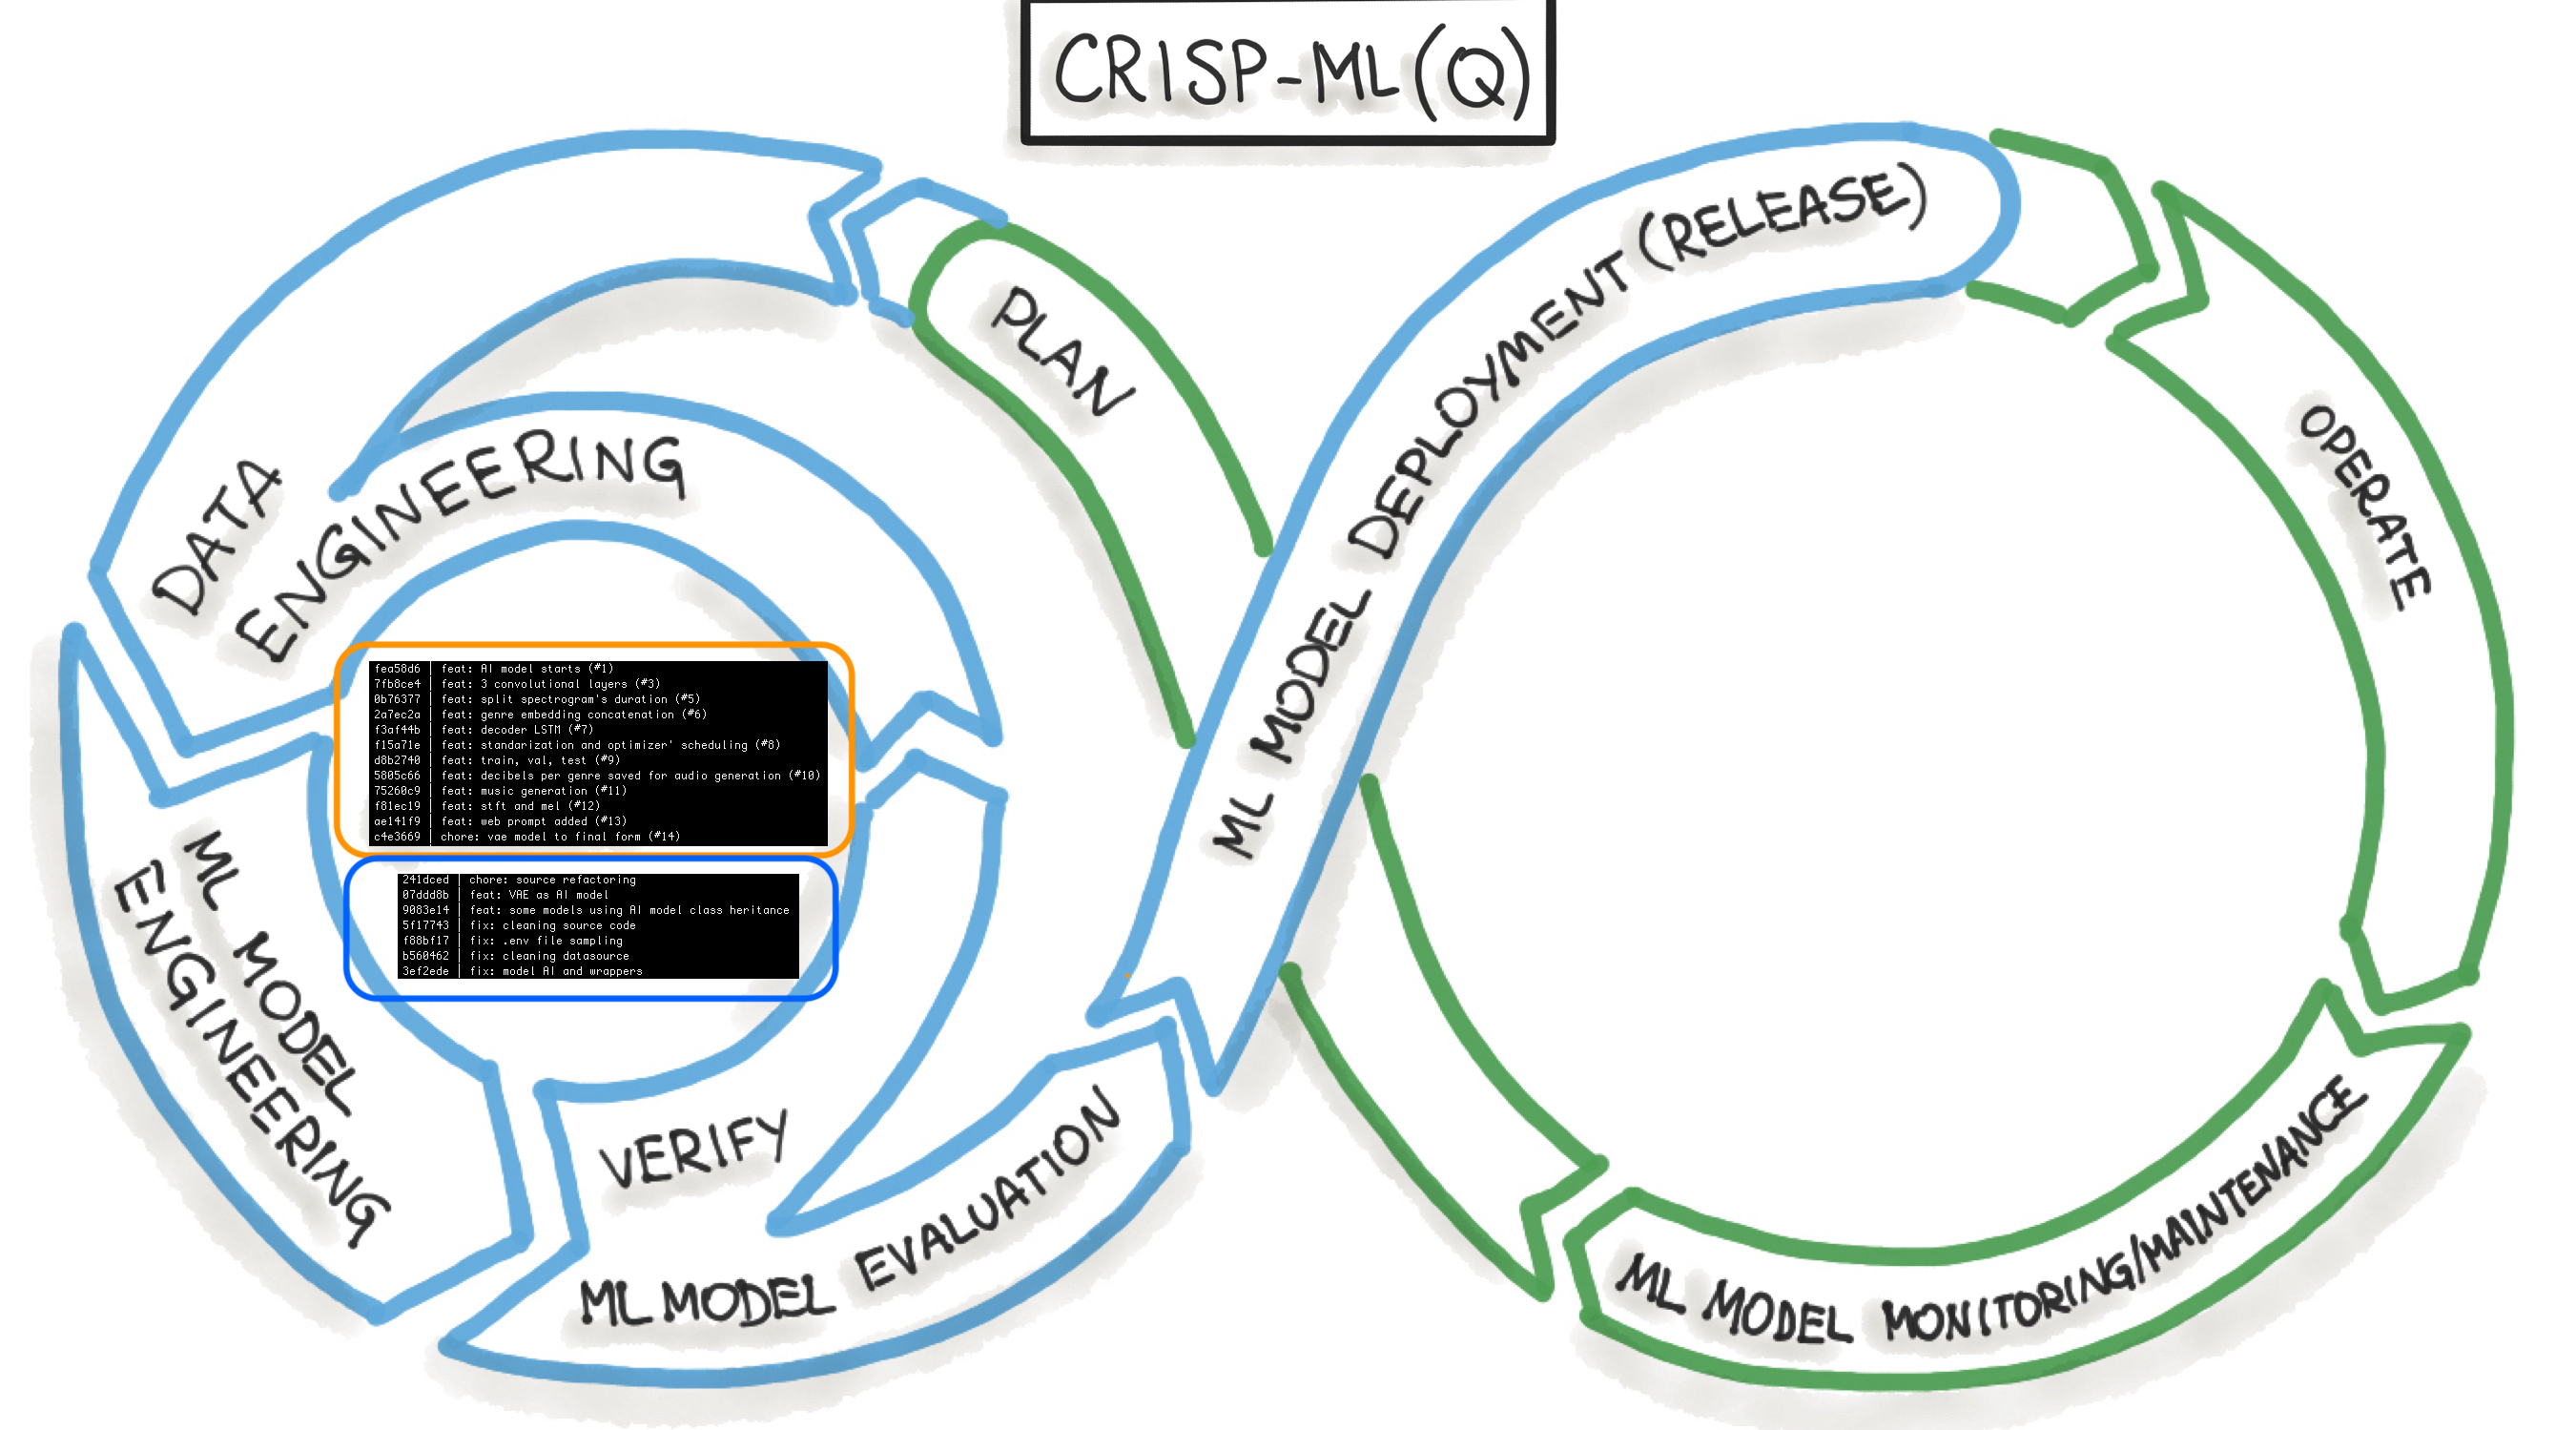
\includegraphics[width=0.9\textwidth]{images/develop-crisp-ml-process.png}
  \end{center}
\end{frame}

\begin{frame}{Metodología}
  \begin{center}
    \textbf{Modelado}: Diagrama de flujo. \textbf{Datos}
  \end{center}
  \begin{center}
    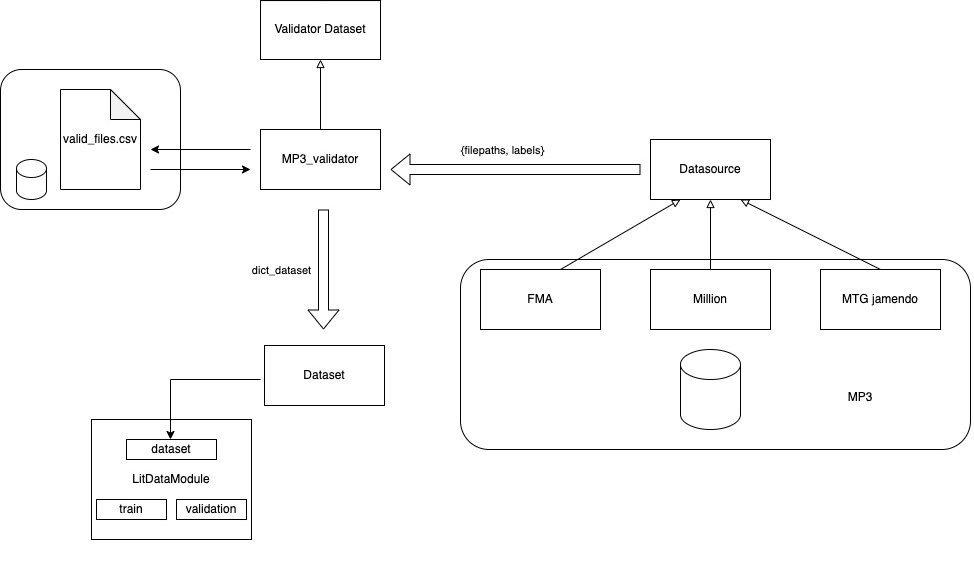
\includegraphics[width=0.9\textwidth]{images/diagrama_flujo_datos.png}
  \end{center}
\end{frame}

\begin{frame}{Metodología}
  \begin{center}
    \textbf{Modelado}: Diagrama de flujo. \textbf{Modelos}
  \end{center}
  \begin{center}
    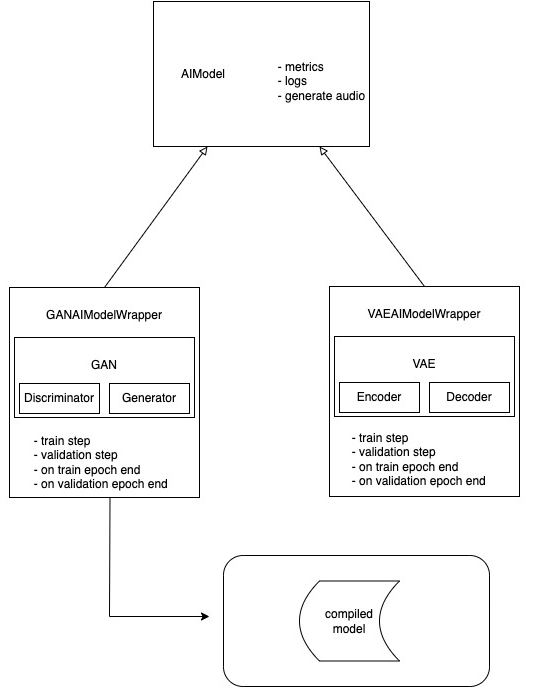
\includegraphics[width=0.4\textwidth]{images/diagrama_flujo_modelos.png}
  \end{center}
\end{frame}

\begin{frame}{Metodología}
  \begin{center}
    \textbf{Modelado}: Diagrama de flujo. \textbf{Test}
  \end{center}
  \begin{center}
    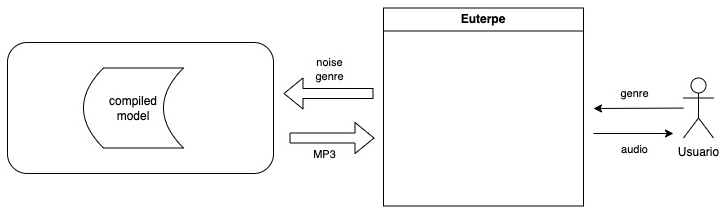
\includegraphics[width=0.7\textwidth]{images/diagrama_flujo_test.png}
  \end{center}
\end{frame}

\begin{frame}{Metodología}
  \begin{center}
    \textbf{Modelado}: Diagrama de flujo. \textbf{Completo}
  \end{center}
  \begin{center}
    \hspace*{0.5cm}\includesvg[width=1\textwidth]{images/diagrama_flujo.svg}
    % 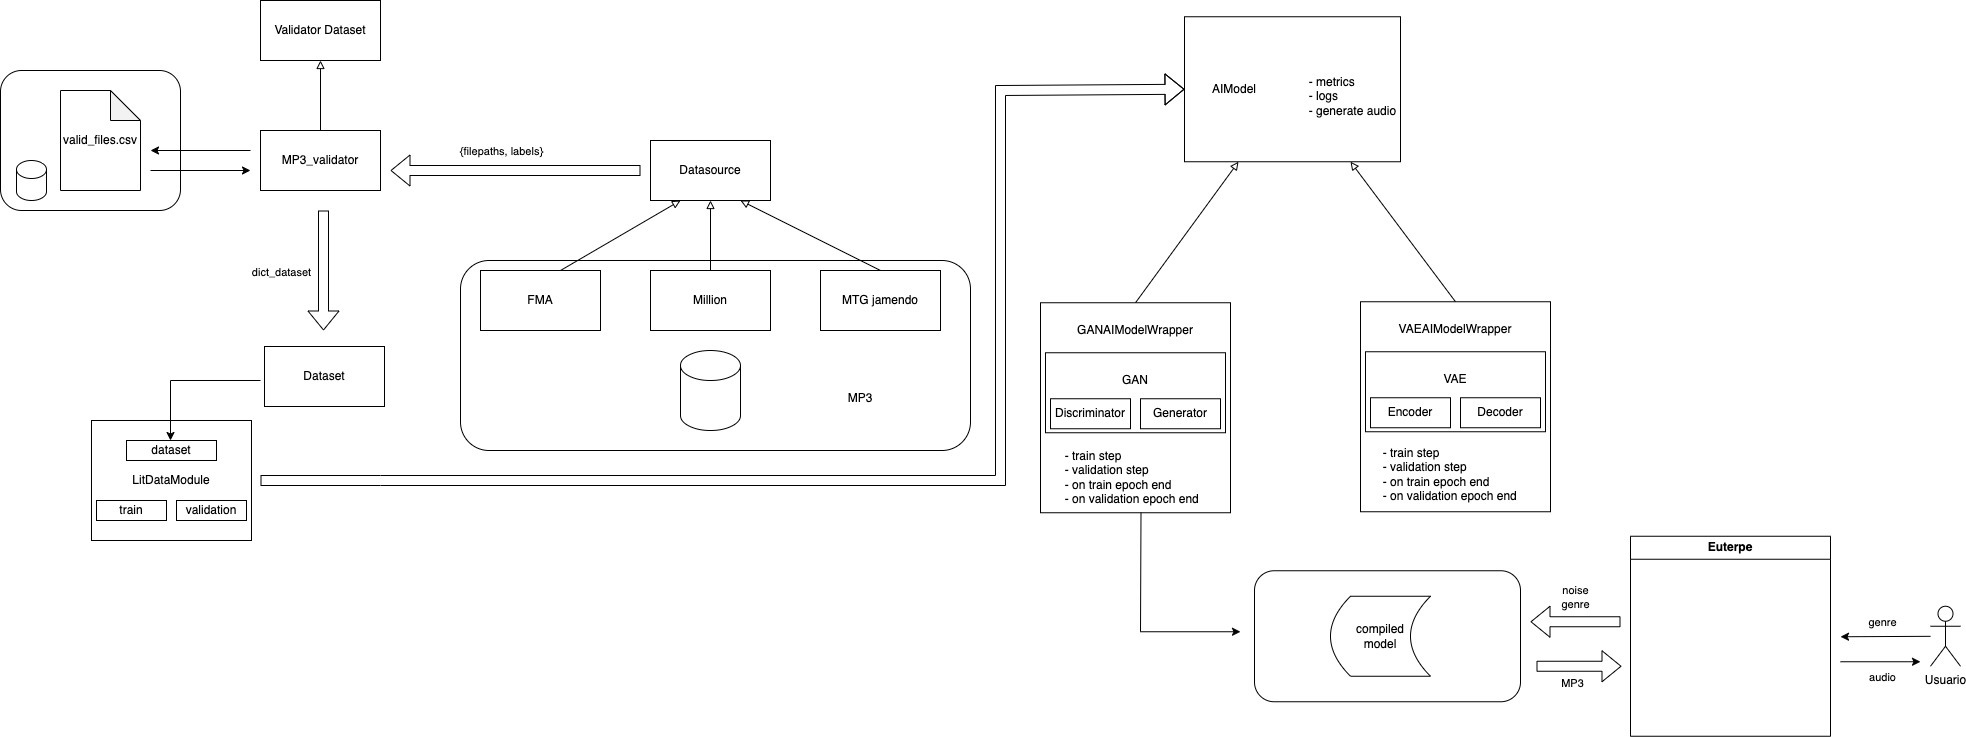
\includegraphics[width=1\textwidth]{images/diagrama_flujo.jpg}
  \end{center}  
\end{frame}


\renewcommand{\currentsectionindex}{5}
\section{Resultados}
\begin{frame}{Resultados VAE}
  % \vspace{-1cm}
  
  \begin{columns}
    \vspace{1cm}
    % \hspace{0.5cm}
    \column{7.5cm}
    
    \begin{center}
      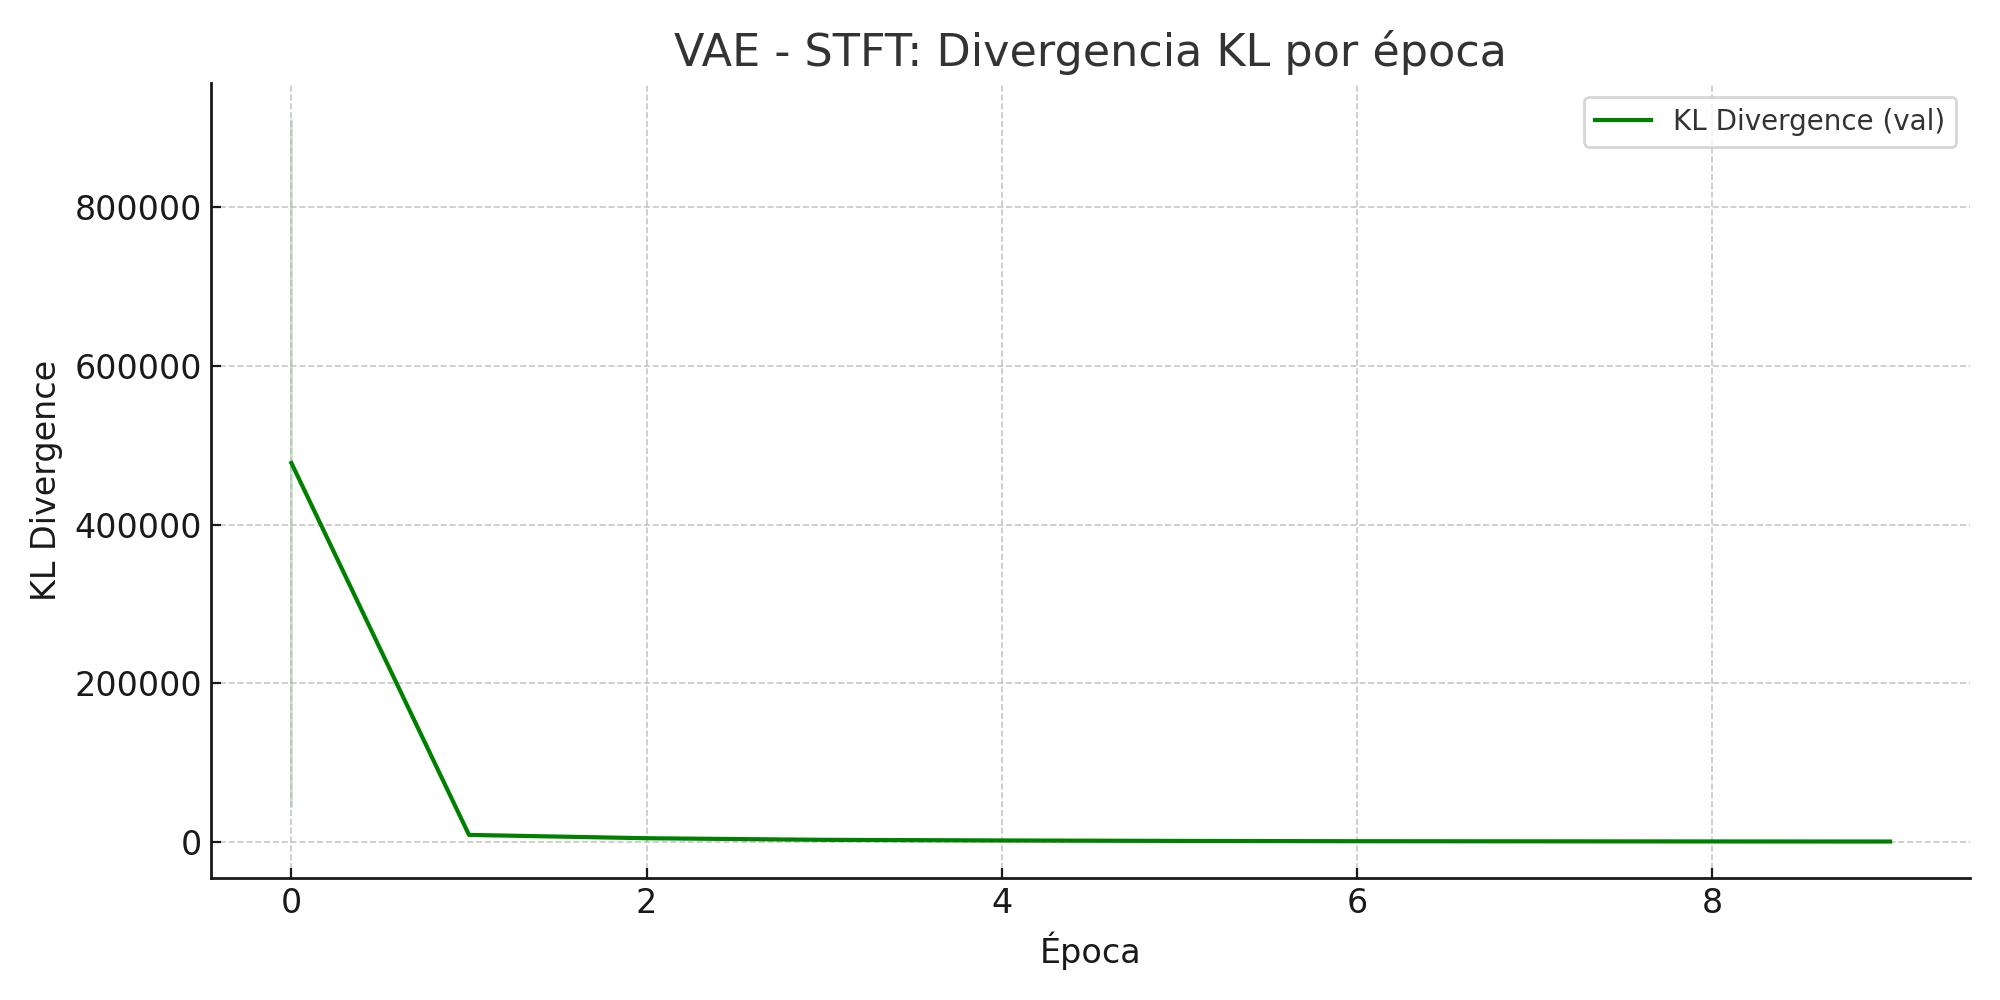
\includegraphics[width=0.8\textwidth]{images/vae_stft_kl_plot.png }
      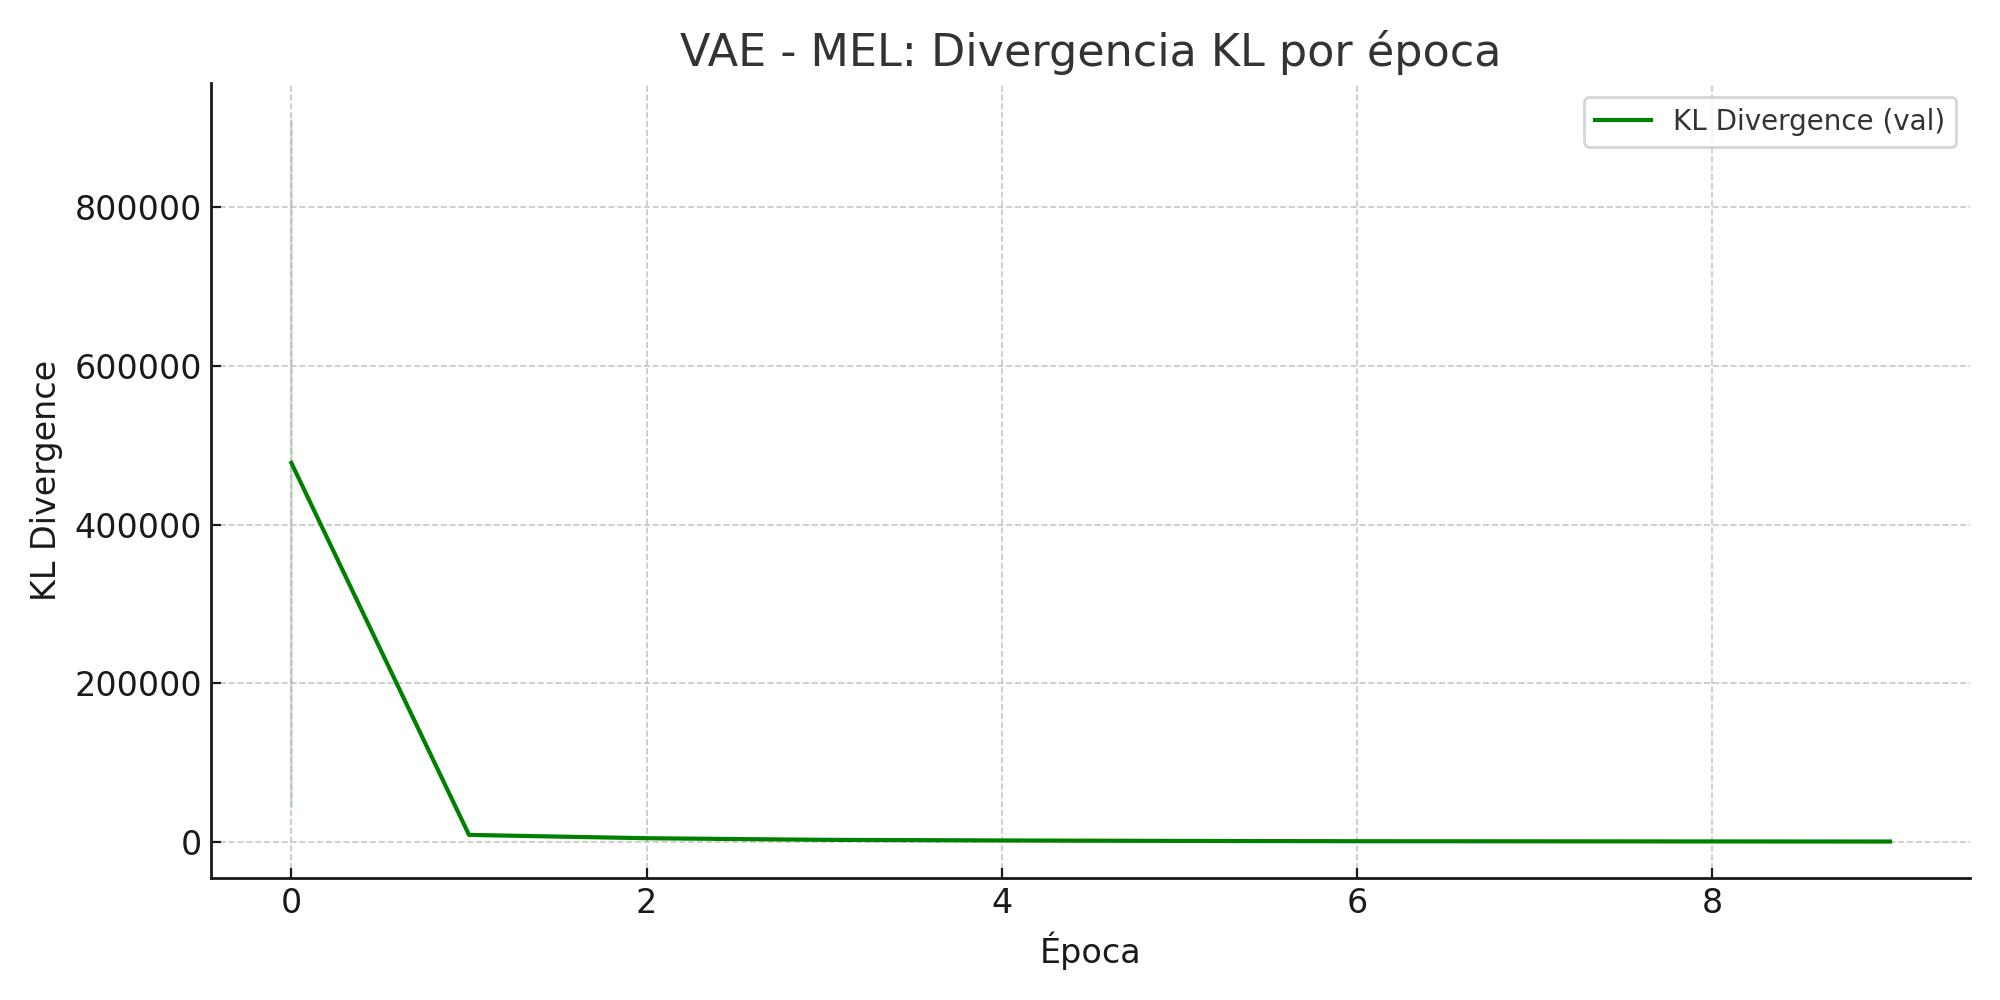
\includegraphics[width=0.8\textwidth]{images/vae_mel_kl_plot.png }
    \end{center}
    \column{4cm}
    \begin{table}
      \centering
      {\fontsize{6pt}{8pt}\selectfont
        \begin{tabular}{rrr}
        epoch & VAE - STFT & VAE - MEL \\
            0 & 5004723.0000 & 911838.0312 \\
            0 &  118500.9789 &  43615.9243 \\
            1 &   19814.0174 &   8572.7893 \\
            2 &    9341.8965 &   4389.1960 \\
            3 &    5147.5633 &   2377.8468 \\
            4 &    3221.6051 &   1579.3012 \\
            5 &    2038.5912 &    997.5138 \\
            6 &    1187.6629 &    624.6872 \\
            7 &     754.9947 &    493.4802 \\
            8 &    3071.2460 &    341.8721 \\
            9 &     338.2404 &    228.3475 \\
        \end{tabular}
      }
    \end{table}
  \end{columns}
\end{frame}

\begin{frame}{Resultados VAE}
  % \vspace{-1cm}
  
  \begin{columns}
    \vspace{1cm}
    % \hspace{0.5cm}
    \column{7.5cm}
    
    \begin{center}
      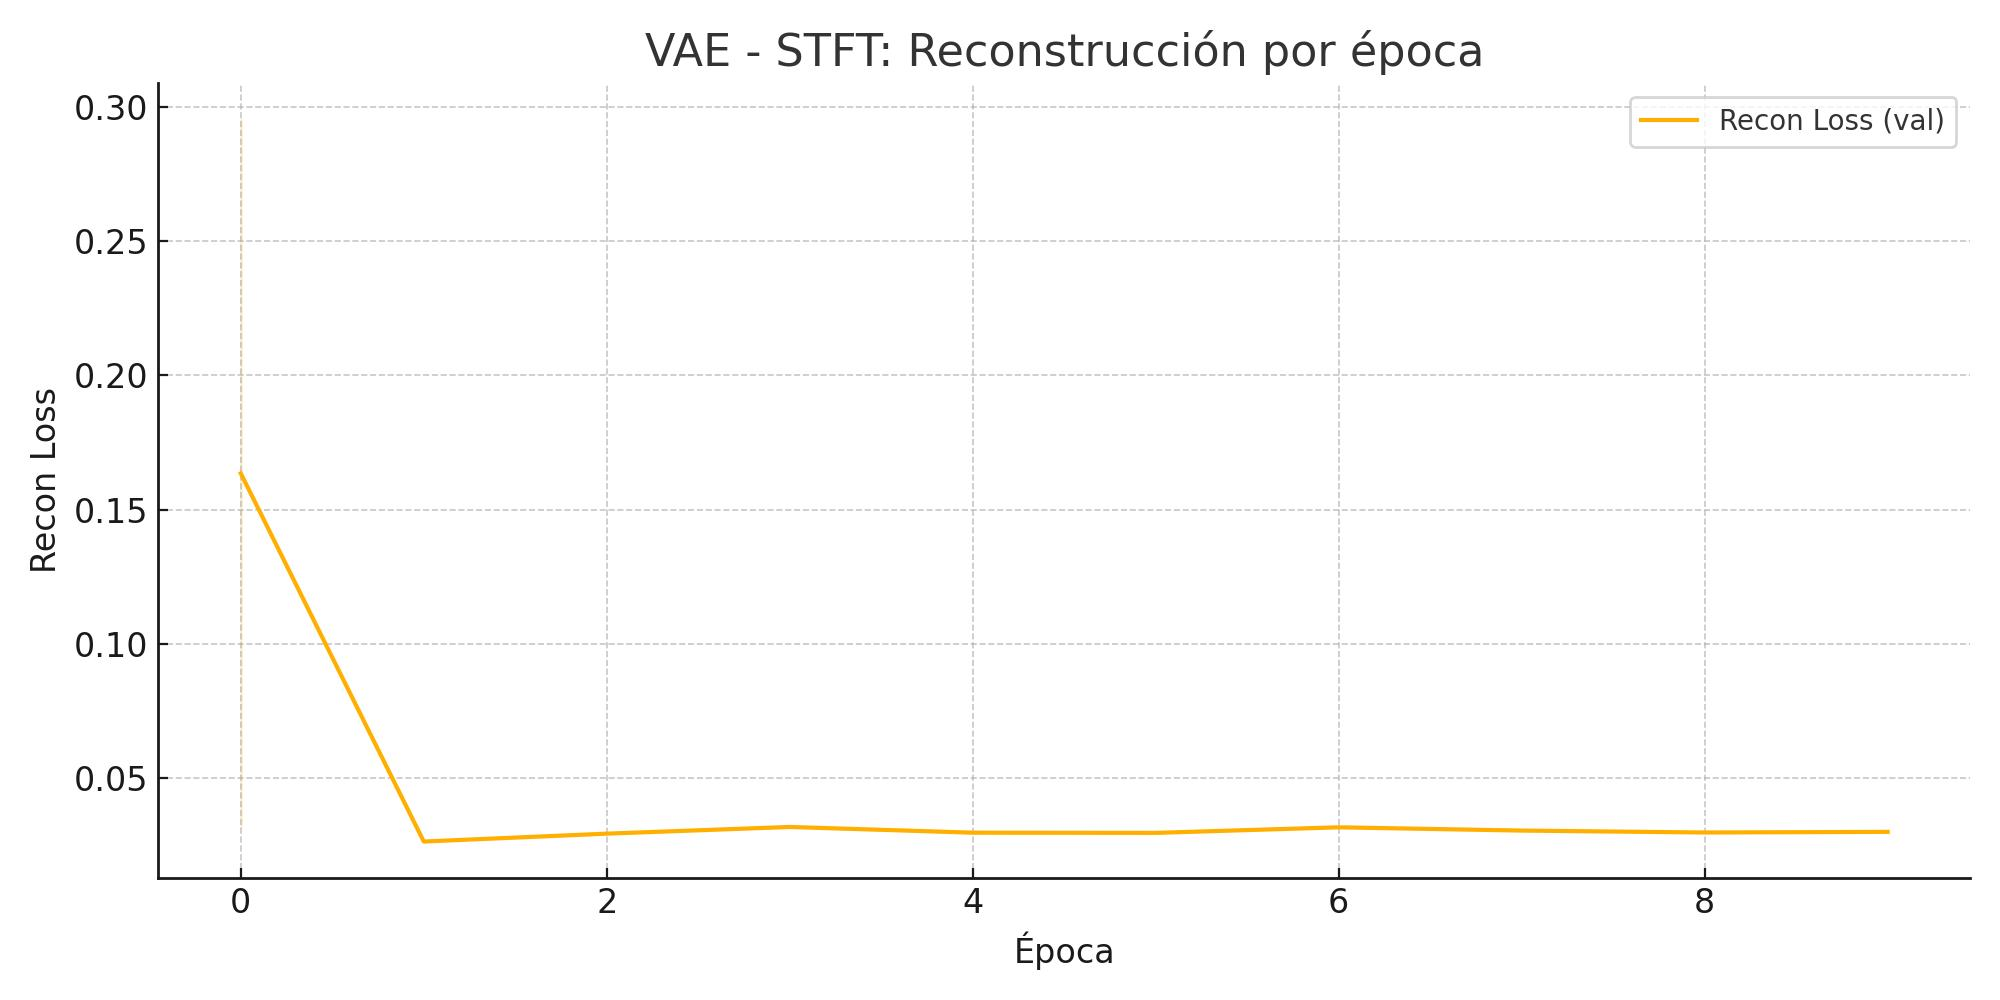
\includegraphics[width=0.8\textwidth]{images/vae_stft_recon_loss_plot.png }
      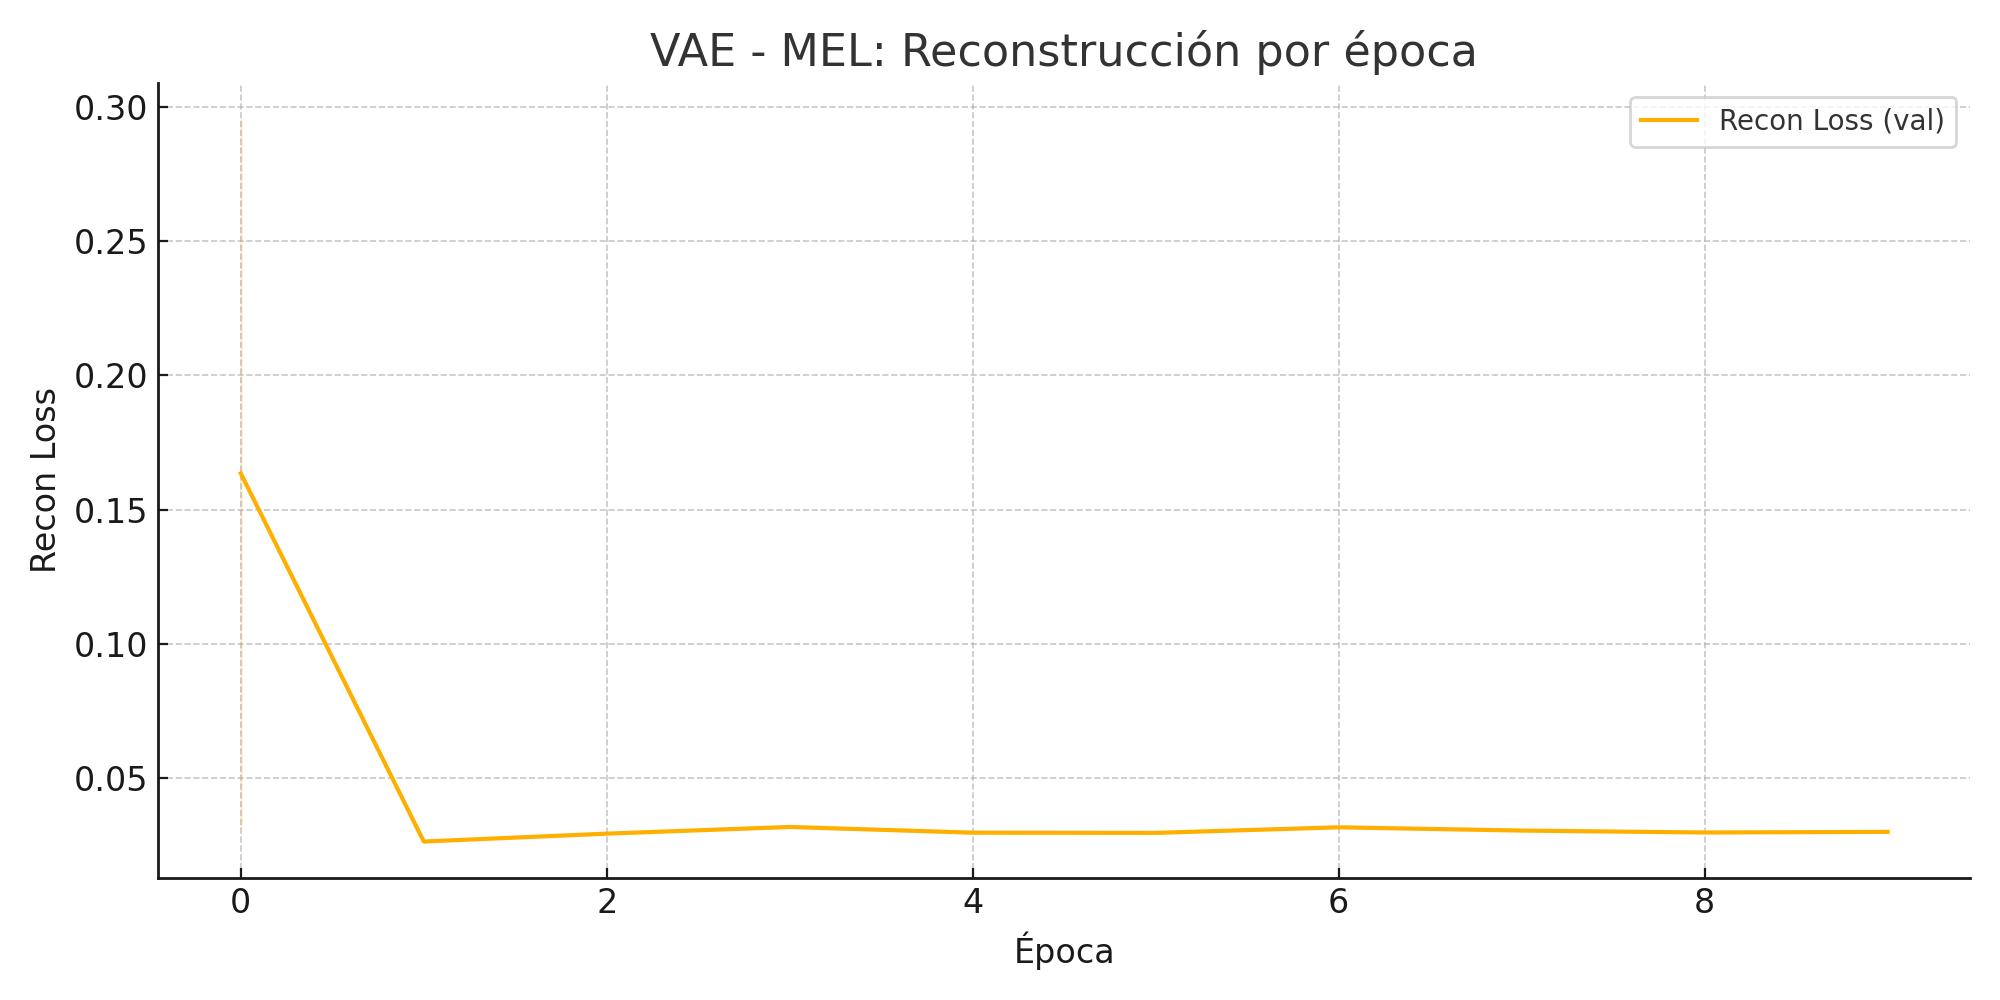
\includegraphics[width=0.8\textwidth]{images/vae_mel_recon_loss_plot.png }
    \end{center}
    \column{4cm}
    \begin{table}
      \centering
      {\fontsize{6pt}{8pt}\selectfont
      \begin{tabular}{rrr}
       epoch & VAE - STFT & VAE - MEL \\
        0 &  0.4259 & 0.2955 \\
        0 &  0.0265 & 0.0315 \\
        1 &  0.0270 & 0.0265 \\
        2 &  0.0297 & 0.0294 \\
        3 &  0.0262 & 0.0319 \\
        4 &  0.0277 & 0.0298 \\
        5 &  0.0262 & 0.0297 \\
        6 &  0.0258 & 0.0318 \\
        7 &  0.0255 & 0.0306 \\
        8 &  0.0343 & 0.0299 \\
        9 &  0.0275 & 0.0301 \\
      \end{tabular}
      } 
      \end{table}
  \end{columns}
\end{frame}

\begin{frame}{Resultados VAE}
  \vspace{-0.4cm}
  \begin{center}
    \textbf{STFT} \\
    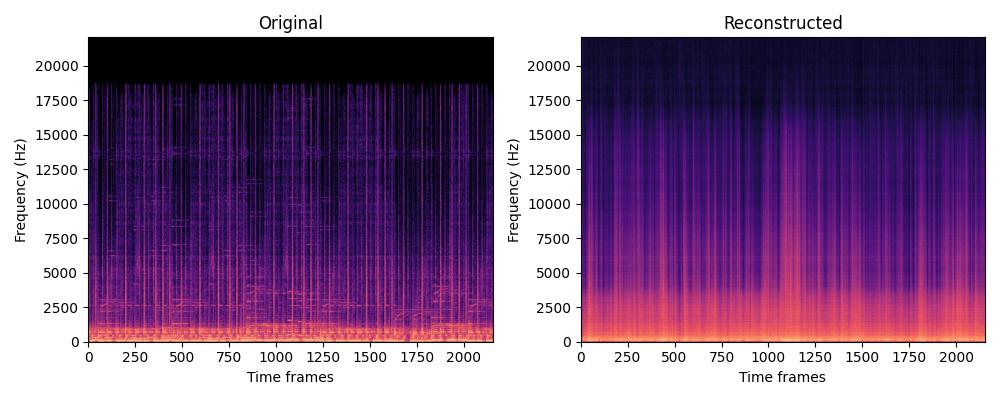
\includegraphics[width=0.7\textwidth]{images/vae_stft_spec_recon.jpg} \\
    \textbf{MEL} \\
    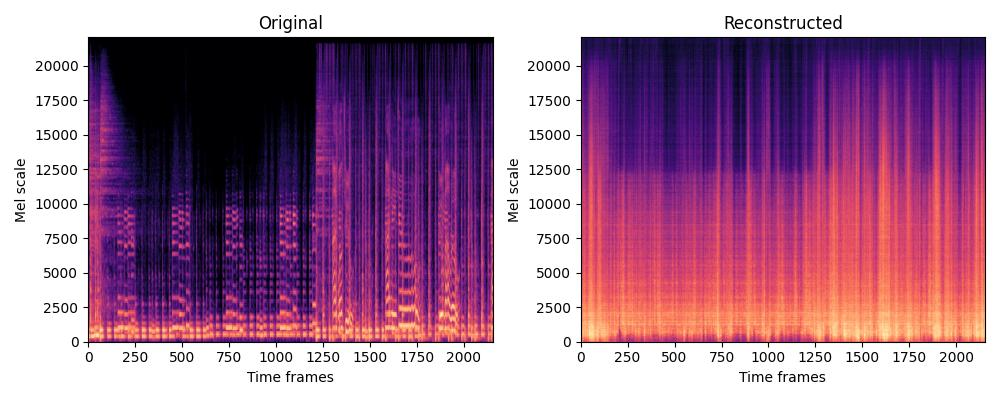
\includegraphics[width=0.7\textwidth]{images/vae_mel_spec_recon.jpg}
  \end{center}
\end{frame}

\begin{frame}{Resultados GAN}
  \begin{center}
    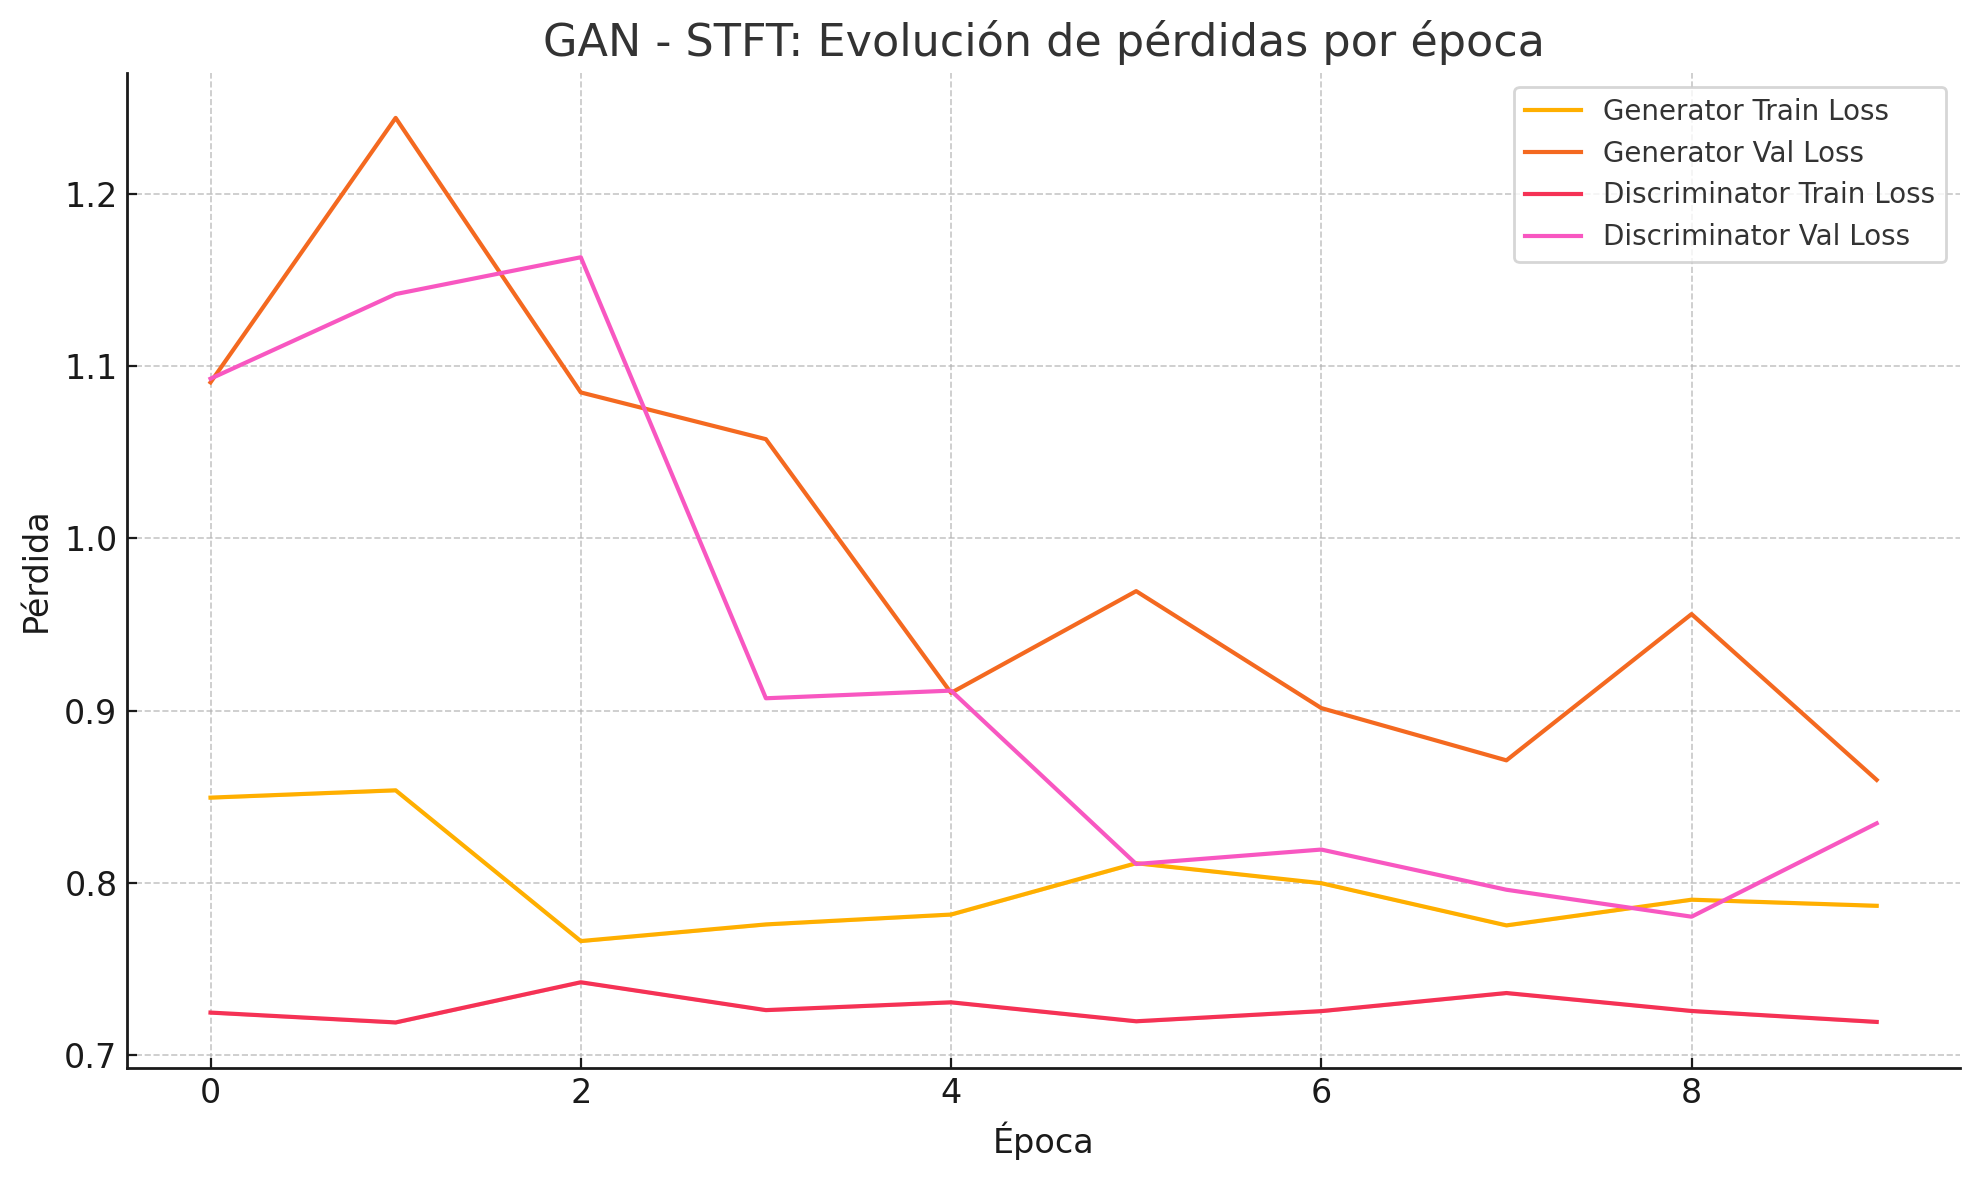
\includegraphics[width=0.5\textwidth]{images/gan_stft_loss_plot.png}
    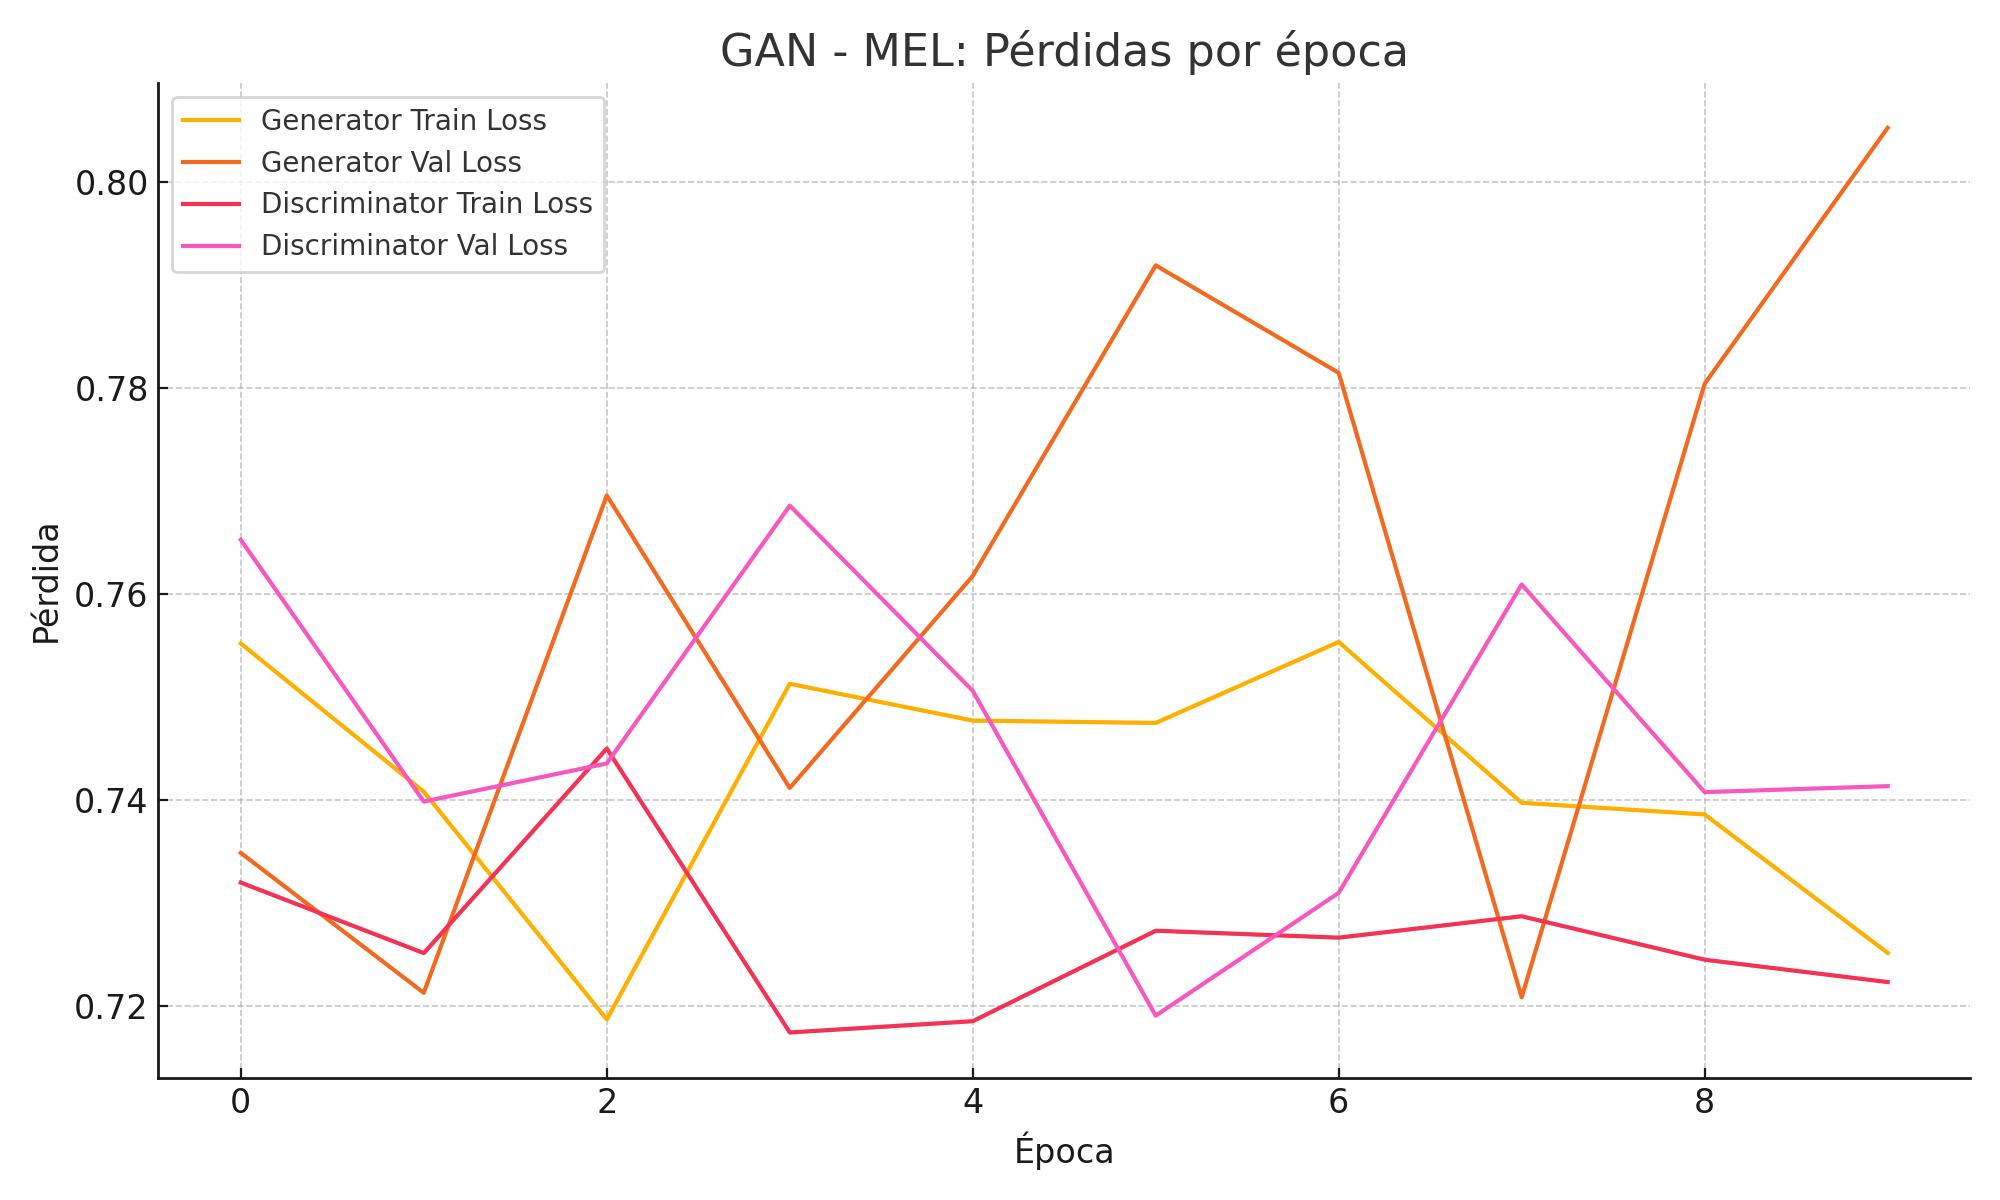
\includegraphics[width=0.5\textwidth]{images/gan_mel_loss_plot.png}
  \end{center}
\end{frame}


\begin{frame}{Resultados GAN}
  \begin{center}
  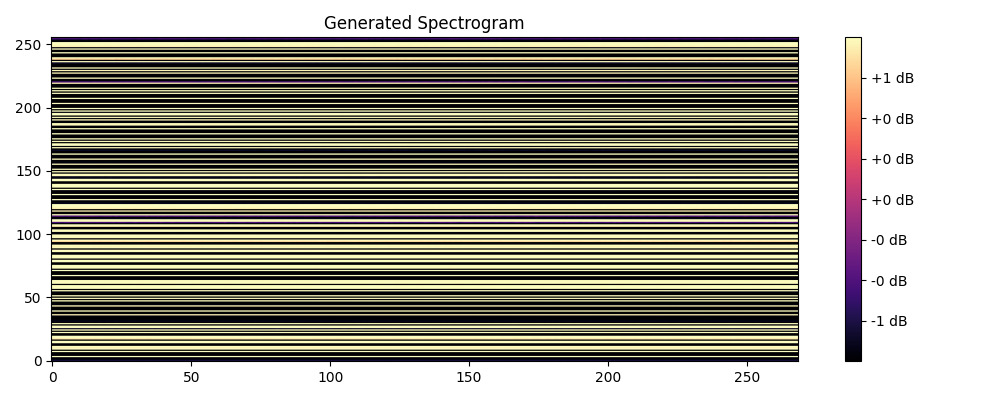
\includegraphics[width=0.9\textwidth]{images/gan_generated_0.jpeg} \\
  \textbf{GAN - MEL - 3 epochs} \\
\end{center}
\end{frame}

\begin{frame}{Resultados GAN}
  \begin{center}
  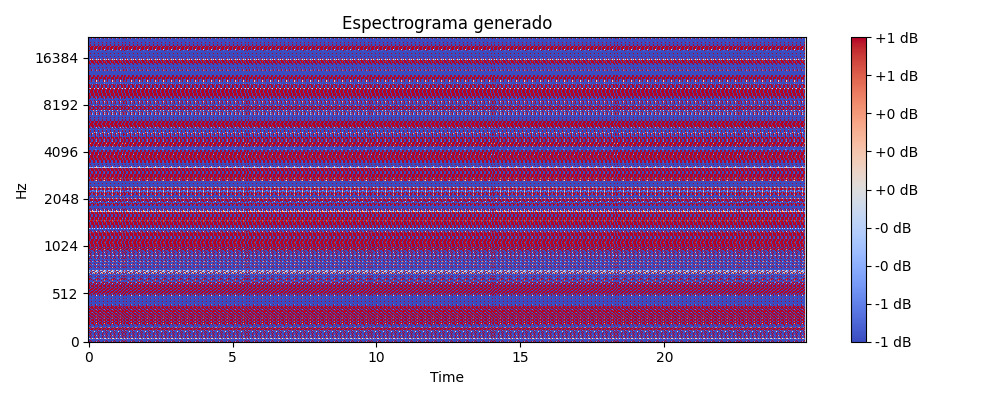
\includegraphics[width=0.9\textwidth]{images/gan_generated_1.jpeg} \\
  \textbf{GAN - MEL - 9 epochs} \\
\end{center}
\end{frame}
\begin{frame}{Resultados GAN}
  \begin{center}
  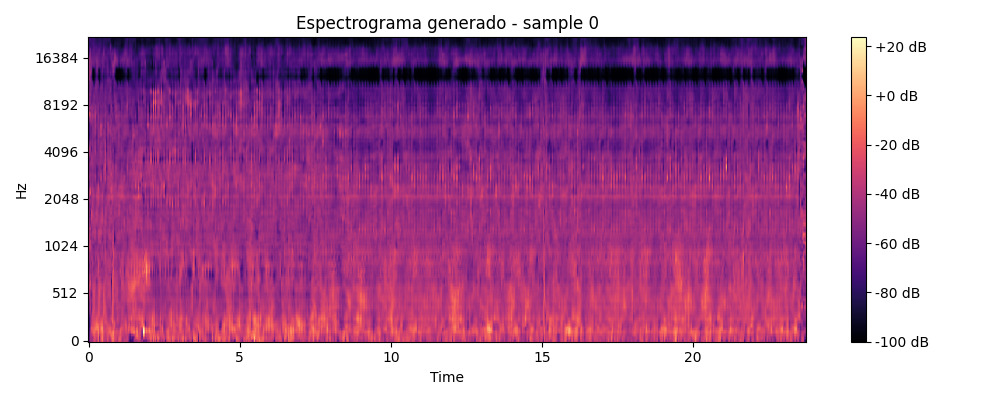
\includegraphics[width=0.9\textwidth]{images/gan_generated_2.jpeg} \\
  \textbf{GAN - MEL - 80 epochs} \\
\end{center}
\end{frame}

\begin{frame}{Resultados GAN}
  \vspace{0.5cm}
  \begin{center}
  \begin{columns}
    \column{5.5cm}
    \hspace*{0.5cm}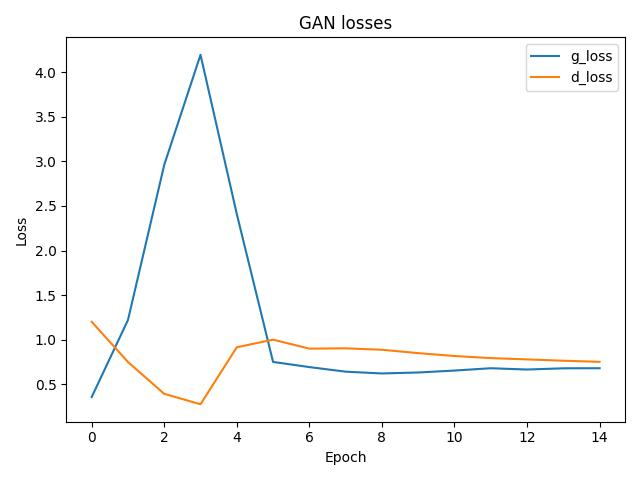
\includegraphics[width=1\textwidth]{images/GAN-loss-14.jpeg}
    \column{5.5cm}
    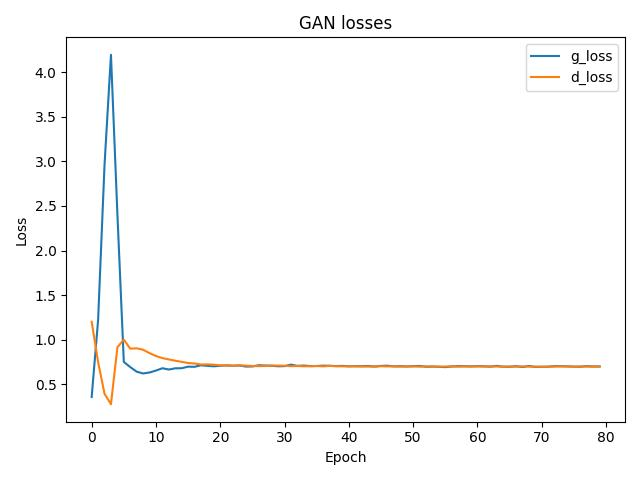
\includegraphics[width=1\textwidth]{images/GAN-loss-80.jpeg}
  \end{columns}
\end{center}
\end{frame}

\begin{frame}{Resultados}
  \vspace{-1cm}
  \begin{center}
  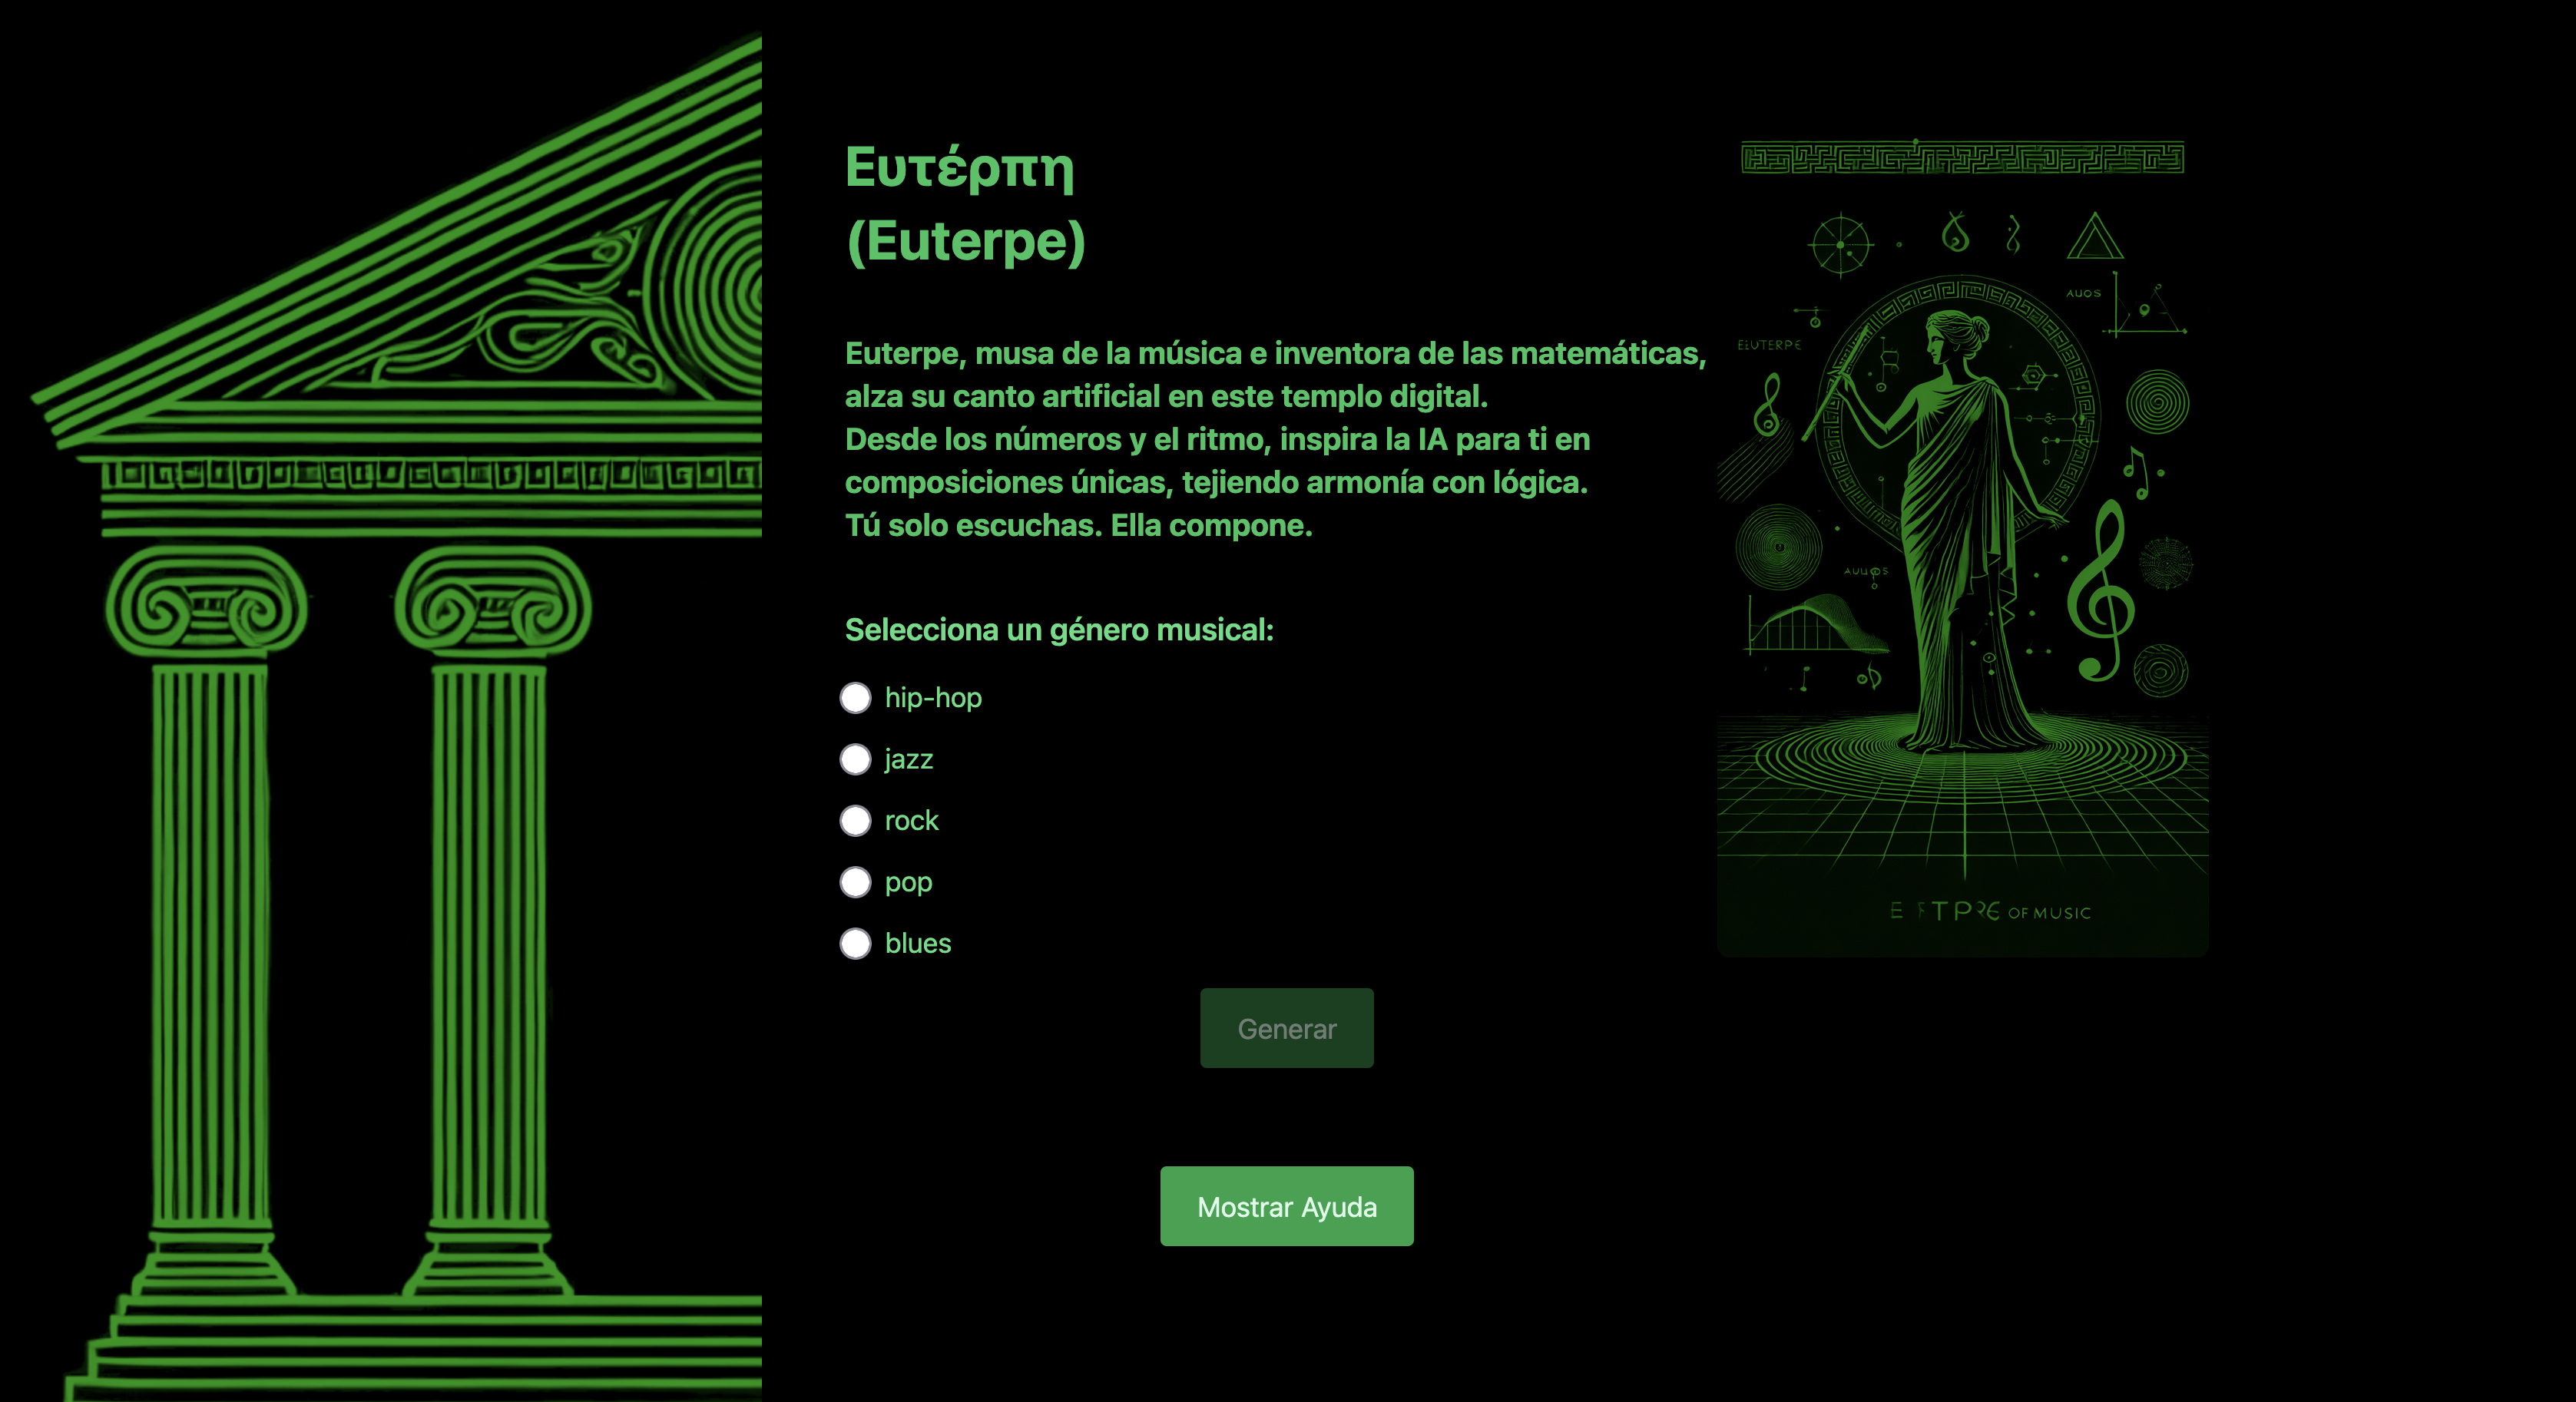
\includegraphics[width=0.9\textwidth]{images/euterpe-screenshot.png}
  \end{center}
\end{frame}



% \begin{frame}{Resultados}
%   \begin{columns}
%     \column{5.5cm}
%     \begin{center}
%       \includegraphics[width=1\textwidth]{}
%     \end{center}
%     \column{6cm}
%     \begin{center}
%       \includegraphics[width=1\textwidth]{}
%     \end{center}
%   \end{columns}
% \end{frame}
 
 



% \begin{frame}{Resultados}
% \end{frame}

% images/gan_mel_losses_epoch_9.jpg 
% images/gan_stft_losses_epoch_9.jpg 
% images/VAE_STFT_mu_hist_step_7950.png

\renewcommand{\currentsectionindex}{6}
\section{Conclusiones}
% \begin{frame}{Conclusiones}
%   \hspace{2cm}
%   \begin{itemize}
%     \item Tratamiento exhaustivo del dataset
%     \item Diseño modular y flexible del sistema de generación musical
%     \item Validación funcional de la arquitectura CNN + LSTM en el entorno VAE
%     \item Implementación del control estilístico mediante condicionamiento por género
%     \item Normalización del espacio latente
%     \item Evaluación de las métricas clave
%     \item Sistema GAN+Transformer
%     \item Aprender
% \end{itemize}
% \end{frame}
\begin{frame}{Conclusiones}
  \hspace{2cm}
  \begin{itemize}
    \item \textbf{Establecimiento de un marco teórico sólido basado en GAN + Transformers}
\end{itemize}
\end{frame}

\begin{frame}{Conclusiones}
  \hspace{2cm}
  \begin{itemize}
    \item \textbf{Establecimiento de un marco teórico sólido basado en GAN + Transformers:}
    \begin{itemize}
      \item GAN: calidad perceptual
      \item Transformers: coherencia temporal
    \end{itemize}
\end{itemize}
\end{frame}

\begin{frame}{Conclusiones}
  \hspace{2cm}
  \begin{itemize}
    \item Establecimiento de un marco teórico sólido basado en GAN + Transformers:
      \begin{itemize}
        \item GAN: calidad perceptual
        \item Transformers: coherencia temporal
      \end{itemize}
    \item \textbf{La metodología CRISP-ML(Q) aseguró un enfoque estructurado desde la comprensión de los datos hasta la evaluación.}
\end{itemize}
\end{frame}

\begin{frame}{Conclusiones}
  \hspace{2cm}
  \begin{itemize}
    \item Establecimiento de un marco teórico sólido basado en GAN + Transformers:
      \begin{itemize}
        \item GAN: calidad perceptual.
        \item Transformers: coherencia temporal.
      \end{itemize}
    \item La metodología CRISP-ML(Q) aseguró un enfoque estructurado desde la comprensión de los datos hasta la evaluación.
    \item \textbf{Se ha creado un ``pipeline'' completo de procesamiento con GAN + Transformers y se ha conseguido identificar aspectos claves para futuras iteraciones sobre este trabajo.}
\end{itemize}
\end{frame}

\begin{frame}{Conclusiones}
  \hspace{2cm}
  \begin{itemize}
    \item Establecimiento de un marco teórico sólido basado en GAN + Transformers:
      \begin{itemize}
        \item GAN: calidad perceptual
        \item Transformers: coherencia temporal
      \end{itemize}
    \item La metodología CRISP-ML(Q) aseguró un enfoque estructurado desde la comprensión de los datos hasta la evaluación.
    \item Se ha creado un ``pipeline'' completo de procesamiento con GAN + Transformers y se ha conseguido identificar aspectos claves para futuras iteraciones sobre este trabajo.
    \item \textbf{El trabajo aporta un análisis riguroso de los desafíos a abordar en generación musical con Inteligencia Artificial y sienta las bases para futuras investigaciones.}
\end{itemize}
\end{frame}

\begin{frame}{Conclusiones}
  \vspace{-1cm}
  \begin{center}
  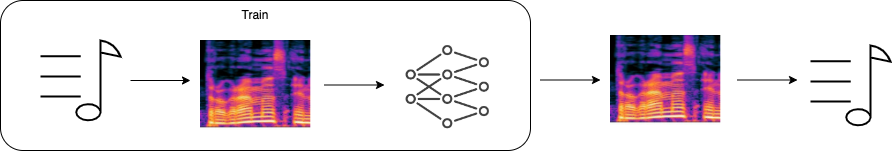
\includegraphics[width=1\textwidth]{images/conversion.png}
  \end{center}
\end{frame}

\begin{frame}{Conclusiones}
  \vspace{0.45cm}
  \begin{center}
  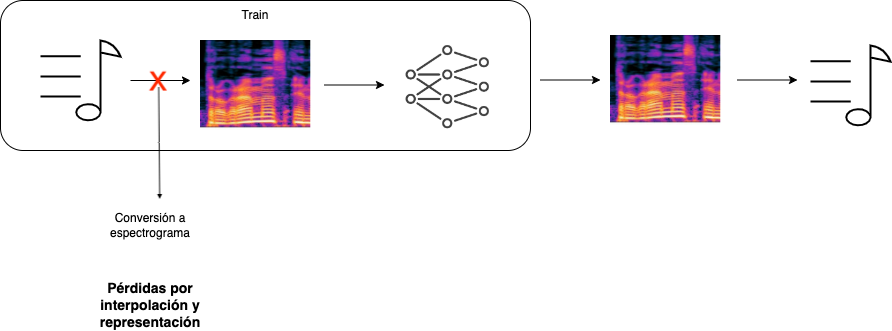
\includegraphics[width=1\textwidth]{images/conversion-fails-1.png}
  \end{center}
\end{frame}

\begin{frame}{Conclusiones}
  \vspace{0.45cm}
  \begin{center}
  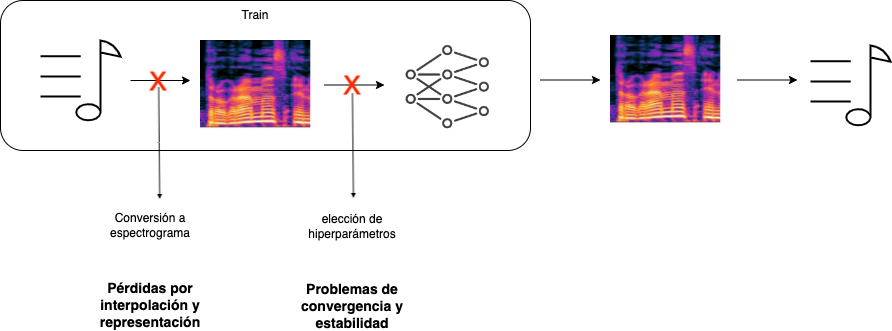
\includegraphics[width=1\textwidth]{images/conversion-fails-2.png}
  \end{center}
\end{frame}

\begin{frame}{Conclusiones}
  \vspace{0.45cm}
  \begin{center}
  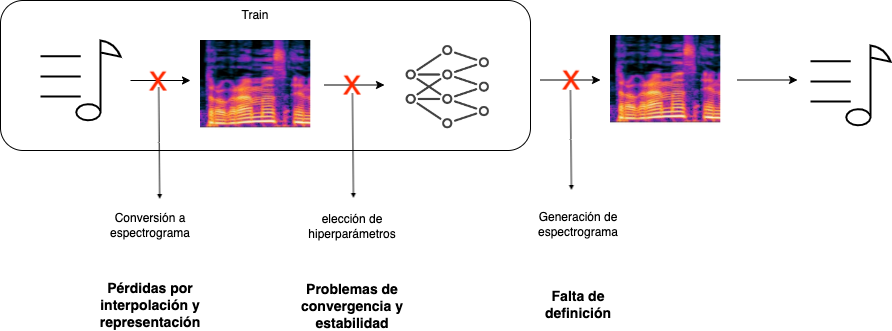
\includegraphics[width=1\textwidth]{images/conversion-fails-3.png}
  \end{center}
\end{frame}

\begin{frame}{Conclusiones}
  \vspace{0.45cm}
  \begin{center}
  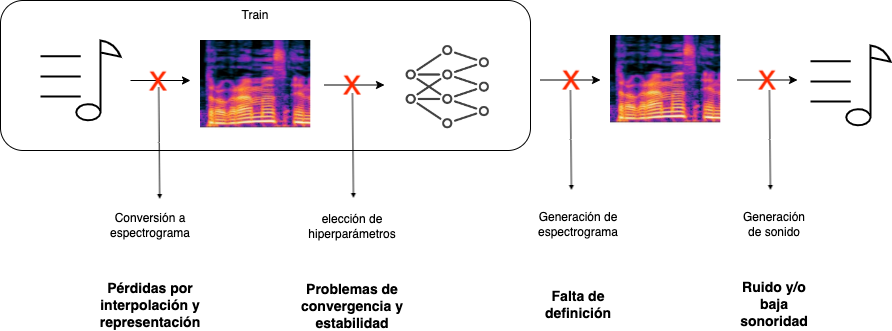
\includegraphics[width=1\textwidth]{images/conversion-fails-4.png}
  \end{center}
\end{frame}

% Si bien no se alcanzaron los resultados esperados, esto se debió a errores inherentes a proyectos pioneros y que ofrecen oportunidades valiosas de aprendizaje.

% Aunque los datasets son robstos, la transformación a espectrogramas, la normalizaci´ón, pudo  introducir artefactos o pérdida de información crítica para el entrenamiento.
% El código presentó errores durante el entrenamiento lo que impidió completar las iteraciones suficientes para que el modelo convergiera y que la elección inicial de hiperparámetros pudo no adaptarse a la complejidad de los datos
% y pudo afectar a la estabilida del modelo



\renewcommand{\currentsectionindex}{7}
\section{Limitaciones}
\begin{frame}{Limitaciones}
  \begin{itemize}
    \item Representación exclusiva mediante espectrogramas STFT o MEL.
    \item Reconstrucción basada en métodos aproximados (Griffin-Lim).
    \item Dependencia del ruido como única fuente de entrada latente.
    \item Limitación del condicionamiento por género.
    \item Dependencia de normalización específica por género.
\end{itemize}
\end{frame}

\renewcommand{\currentsectionindex}{8}
\section{Trabajos futuros}
\begin{frame}{Trabajos futuros}
  \begin{itemize}
  \item Composiciones ``domésticas''
  \item Bases musicales para:
    \begin{itemize}
      \item músicos profesionales
      \item videojuegos
      \item personalización de dispositivos
    \end{itemize}
    \item Ética y legislación (propiedad)
    \item Modelos híbridos
    \item Involucrar músicos profesionales para evaluar resultados
  \end{itemize}
\end{frame}

\begin{frame}
  \vspace{2cm}
  \begin{columns}
    % \column{5cm}
    % \column{5.5cm}
    \column{12cm}
    \begin{flushright}
      \emph{El silencio en la música equivale al lienzo en blanco en la pintura.}\\
    \end{flushright}
    \vspace{0.5cm}
    \begin{flushright}
      Gonzalo Cabrera Peña.
    \end{flushright}
  \end{columns}
  \vspace{1cm}
  \begin{center}
    
\includegraphics[width=3cm]{images/viu_logo.png}
  \end{center} 
\end{frame}

\end{document}
